\documentclass{article}

\usepackage{geometry}
\usepackage{makecell}
\usepackage{array}
\usepackage{multicol}
\usepackage{xcolor}
\usepackage{nicefrac}
\usepackage{amsmath}
\usepackage{amssymb}
\usepackage{hyperref}
\usepackage{setspace}
\usepackage[explicit]{titlesec}
\usepackage{changepage}
\usepackage{booktabs}
\usepackage{graphicx}
\usepackage{float}
\newcolumntype{?}{!{\vrule width 1pt}}
\renewcommand\theadalign{tl}
\renewcommand{\contentsname}{Inhaltsverzeichnis:}
\newcommand{\paragraphlb}[1]{\paragraph{#1}\mbox{}\\}
\newcommand{\N}{\mathbb{N}}
\newcommand{\tto}{\ensuremath{\to}}
\setstretch{1.10}
\setlength{\parindent}{0pt}
\definecolor{grey}{HTML}{808080} 

\titleformat{\section}
  {\normalfont\Large\bfseries}{\thesection}{1em}{\hyperlink{sec-\thesection}{#1}
\addtocontents{toc}{\protect\hypertarget{sec-\thesection}{}}}
\titleformat{name=\section,numberless}
  {\normalfont\Large\bfseries}{}{0pt}{#1}

\titleformat{\subsection}
  {\normalfont\large\bfseries}{\thesubsection}{1em}{\hyperlink{subsec-\thesubsection}{#1}
\addtocontents{toc}{\protect\hypertarget{subsec-\thesubsection}{}}}
\titleformat{name=\subsection,numberless}
  {\normalfont\large\bfseries}{\thesubsection}{0pt}{#1}

\hypersetup{
    colorlinks,
    citecolor=black,
    filecolor=black,
    linkcolor=black,
    urlcolor=black
}
\geometry{top=12mm, left=1cm, right=2cm}
\title{\vspace{-1cm}Grundlagen der Informatik 1}
\author{Andreas Hofer}

\begin{document}
	\maketitle
	\tableofcontents
	\newpage
	\section{Einleitung}
	Grundsätzlich muss man zwischen analogen und digitalen Rechnern unterscheiden. Analoge Rechner benützen stufenlose Werte zur Berechnung von Ergebnissen, mit einer kontinuierlichen Skala. Ein Rechenschieber ist Beispiel für einen analogen Rechner. Dem gegenüber stehen digitale Rechner, welche mit diskreten Werten arbeiten und nur 1 oder 0 verarbeiten können und dabei verschiedene Zustände verwenden um diese zu interpretieren. Ein Abakus ist Beispiel einer digitalen Rechenmaschine (auch wenn sie nicht sehr digital erscheinen mag).
	\begin{figure}[H]
	\centering
	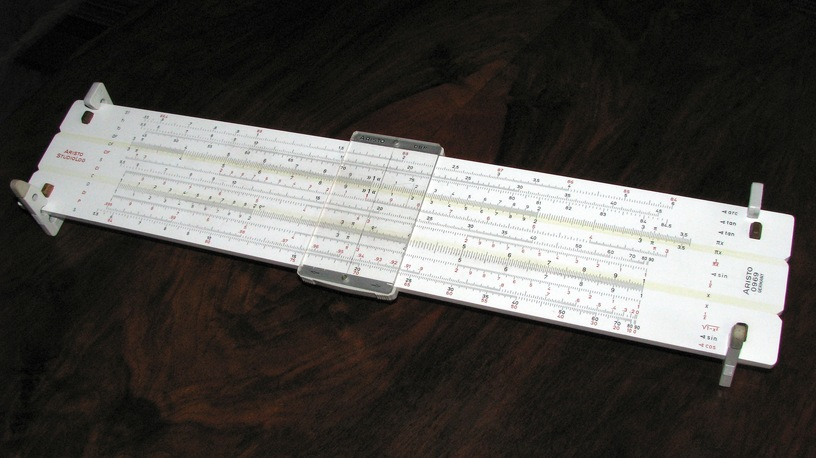
\includegraphics[scale=0.78]{Bilder/smol_rechenschieber.jpg}
	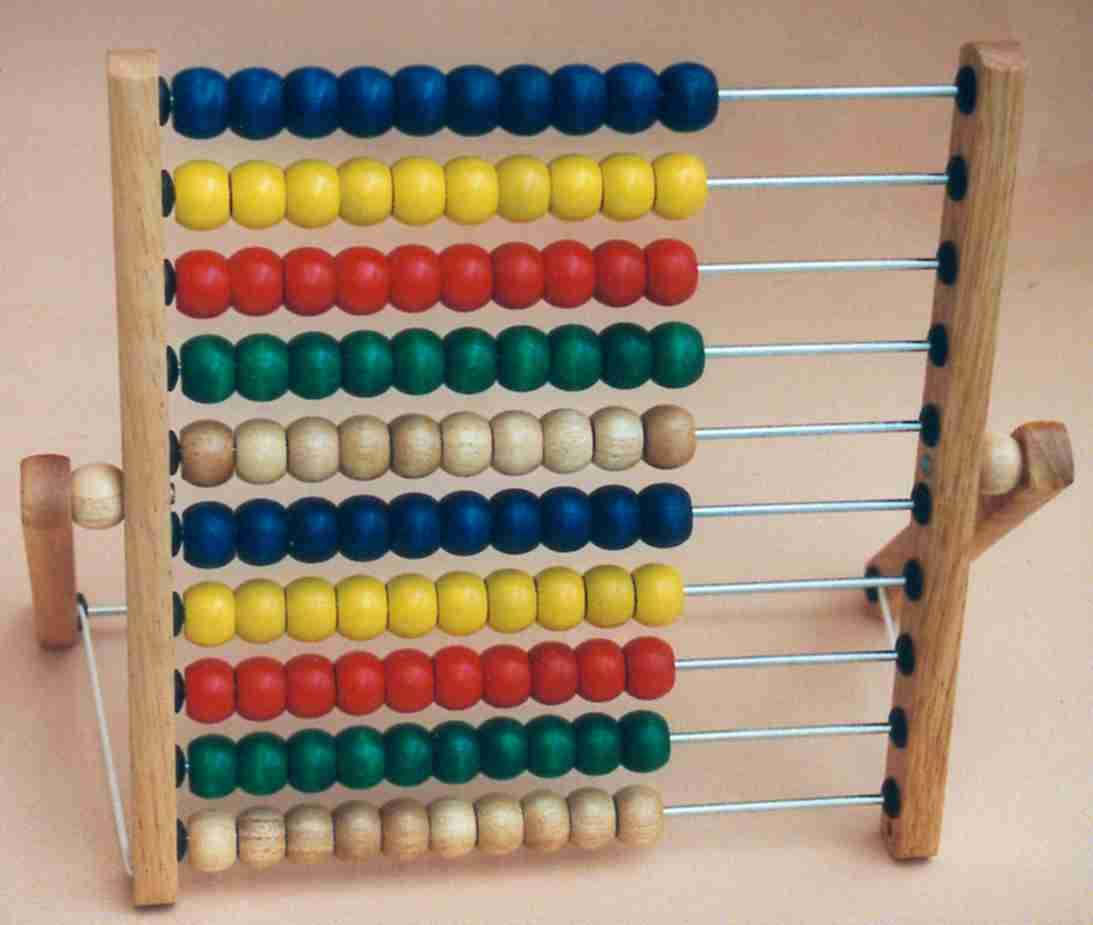
\includegraphics[scale=0.165]{Bilder/abakus.jpg}
	\caption{Rechenschieber vs. Abakus}
	\end{figure}
	\subsection{Geschichtlicher Überblick}
	Während ihrer Geschichte wurden verschiedene Medien verwendet um die Berechnungen auf einer Rechenmaschine zu vollbringen. Die wichtigsten hierbei sind: 
	\begin{itemize}
		\item{Schalter}
		\begin{itemize}
			\item{Ein Relais, welches mechanisch einen Stromfluss unterbricht oder zulässt.}
		\end{itemize}
		\item{Vakuumröhren}
		\begin{itemize}
			\item{Erster rein digitaler Schalter mit einer bedeutend höheren Geschwindigkeit als Relais.}
			\item{Verbrauchen jedoch große Mengen an Energie und sind relativ fehleranfällig.}
		\end{itemize}
		\item{Transistor}
		\begin{itemize}
			\item{Halbleiter, welche abhängig von ihrer Konfiguration einen Stromfluss erlauben oder nicht.}
			\item{Sind kleiner, effizienter, schneller und weniger fehleranfällig als Vakuumröhren.}
		\end{itemize}
		\item{Integrierte Schaltkreise}
		\begin{itemize}
			\item{Verbundene Schaltkreise, welche aus vielen Transistoren bestehen.}
		\end{itemize}
	\end{itemize}
	Gottfried Wilhelm Leibnitz erfand 1694 die erste Rechenmaschine, da er der Ansicht war, dass 'Menschen nicht gleich Sklaven niedere Rechenarbeiten tätigen sollten'. Seine Maschine beherrschte die vier Grundrechnungsarten indem Zahnräder und Walzen sich drehten und dabei die Berechnungen durchführten. \\
	Etwas später, 1873 erfand Charles Babbage die \textit{Analytical Engine}, welche die erste universelle Rechenmaschine war und dadurch mehr als die vier Grundrechnungsarten beherrschte. Diese Maschine soll auch programmierbar gewesen sein, wobei Ada Lovelace als erste Person gilt, welche ein solches Programm schrieb. \\
	Noch später, 1890 entwickelte Herman Hallerith die \textit{Tabulating Machine}. Diese sollte bei der Auswertung der Volkszählung in den USA helfen indem Lochkarten die Eigenschaften der verschiedenen Personen festhielten, und dadurch nur mehr von ihr ausgewertet werden mussten. Das hatte zur Folge, dass es statt 8 Jahren für die Volkszählung 1880 nur 6 Jahre zur Vollendung brauchte, wobei 25\% mehr Personen gezählt wurden. Diese Maschine fand auch später in Firmen zur Buchhaltung Anwendung. \\
	Die erste universell programmierbare, digitale Rechenmaschine wurde 1941 von Konrad Zuse entwickelt. Er entwickelte auch 'Plankalkül', die erste high-level Programmiersprache, diese wurde jedoch nie angewendet. \\
	Unabhängig davon baute die Universität Harvard 1944 die Harvard Mark 1 um Berechnungen für das Manhatten Project zu vereinfachen. \\
	Bereits ein Jahr später bauten John Mauchly und J. Presper Eckert die ENIAC (Electronic Numerical Integrator and Computer), welcher der erste universell programmierbare, elektronische, digitale Rechner war. Durch die austauschbare physische Verkabelung konnte man ihn zwar programmieren, jedoch keine Programme speichern. \\
	Zur gleichen Zeit entwickelte John von Neumann die \textit{von Neumann Architektur}, welche sowohl den Programmcode, als auch die zu verarbeitenden Daten im gleichen Speicher halten sollte um so Platzeffizienter agieren zu können. \\
	Nach dem Erfolg des ENIAC, gründeten Eckert und Mauchly die \textit{Eckert-Mauchly Computer Corporation} um Rechenmaschinen komerziell verfügbar zu machen. Ihr größter Erfolg war das UNIVAC (Universal Automatic Computer), welcher als erste kommerziell verfügbarer Computer gilt, anders als der ENIAC nun jedoch Magnetbänder als Speichermedium verwendet.\\
	Die Apollo Mission 1960 gilt als die erste Mission die integrierte Schaltkreise verwendete. \\
	1969 wurde das ARPANET (Advanced Research Projects Agency Network) erstmals verbunden, welches als Vorgängerkomponente des modernen Internets gilt. \\
	In den 70er-Jahren nahmen die Fortschritte in der Computertechnologie rasant zu. Intel entwickelte den Intel 4004, was der erste kommerziell erhältliche Mikrochip war. Zur gleichen Zeit wird auch UNICS, heute bekannt als UNIX, entwickelt. Ebenfalls kommt der ALTAIR 8800 auf den Markt, der erste komerziell verfügbare PC. Es war dieser PC für den Bill Gates 1975 ALTAIR Basic schrieb, welches das erste von Microsoft verkaufte Produkt war.
	\section{Informationsdarstellung}
	Ein Computer hat drei grundlegende Aufgaben: Eingabe, Verarbeitung und Ausgabe. Das nennt man das EVA-Prinzip. Dabei sollen sie über eine Schnittstelle Informationen einlesen und akzeptieren, diese intern verarbeiten und/oder speichern und bei Bedarf wieder ausgeben. Jegliche Information die von einem Computer verarbeitet wird, muss jedoch zuerst in das Binärsystem umgewandelt werden.
	\subsection{Binärsystem}
	Das Binärsystem, auch Dualsystem genannt, kennt nur zwei Zahlen: 0 und 1. Diese stellen jeweils einen diskreten Wert dar, wodurch jedes System das Binärzahlen verwendet, ein digitales System ist. So werden Vakuumröhren, oder Relais oder Halbleiter verwendet um diese beiden diskreten Werte jeweils darzustellen. Innerhalb eines PCs nennt man diese kleinstmögliche Informationseinheit ein \textbf{Bi}nary Digi\textbf{t}, oder kurz Bit. Ein Computer interpretiert Bits in der realen Welt auf verschiedene Weisen. Zum Beispiel wird bei Halbleitern überprüft ob eine gewisse Spannung präsent ist und interpretiert dies als 0, falls es nicht zutrifft. Man kann mit Bits jedoch nicht nur einen einzigen Zustand darstellen. Wenn man mehrere Bits aneinanderreiht, können diese viel mehr einzigartige Zustände darstellen und so mehr Informationen speichern. Bitfolgen haben die Eigenschaft, dass sie mit jedem hinzugefügten Bit die mögliche Anzahl der Zustände verdoppeln. Aus diesem Grund kann man die Anzahl der möglichen Zustände mittels $2^n$ berechnen, wobei n die Anzahl der zur Verfügung stehenden Bits ist. Durch die sich verdoppelnde Anzahl kann man selbst mit einem so elementaren Werkzeug irgendwann eine sehr große Menge an Zuständen abbilden. Bei 32 Bits und $2^{32}$Zuständen sind das bereits 4.294.967.296 die abgebildet werden können. Daten werden jedoch selten in Bits angesehen und werden stattdessen in Gruppen von 8 Bits geteilt, welche man Bytes nennt. \verb|1 Byte -> 8 Bit|. Diese werden wiederum in Blöcke von jeweils 1024 geteilt. So nennt man 1024 Bytes 1 Kilobyte und 1024 Kilobyte 1 Megabyte usw. Durch den Umstand, dass bei jeder Gruppierung jedoch 24 Byte extra genommen werden, kann dieses System im täglichen Sprachgebrauch ungenau sein. Wenn man normalerweise von 'Einem Terabyte' spricht meint man 1000 Gigabyte, oder 1.000.000 Megabyte, was jedoch als Zweierpotenz 1.099.511 Megabyte sind. Dadurch entsteht eine Diskrepanz, welche größer wird, je größer die Nummer ist. So entspricht sie hier etwa 10\% während es bei einem Yottabyte ($2^{80}$) schon 20\% sind: \\
	\begin{tabular}{| l | c l | c  l | l |}
		\toprule
		Name & Exponent & Bytes & Exponent & Bytes & Diskrepanz \\ \midrule
		Kilobyte & $2^{10}$ & 1.024 & $10^3$ & 1.000 & 2,4\% \\ \hline
		Megabyte & $2^{20}$ & 1.048.576 & $10^6$ & 1.000.000 & 4,8\% \\ \hline
		Gigabyte & $2^{30}$ & 1.073.741.824 & $10^9$ & 1.000.000.000 & 7,3\% \\ \hline
		Terabyte & $2^{40}$ & 1.099.511.627.776 & $10^{12}$ & 1.000.000.000.000 & 9,9\% \\ \hline
		Petabyte & $2^{50}$ & 1.125.899.906.842.624 & $10^{15}$ & 1.000.000.000.000.000 & 12,5\% \\ \hline
		Exabyte & $2^{60}$ & 1.152.921.504.606.846.976 & $10^{18}$ & 1.000.000.000.000.000.000 & 15,2\% \\ \hline
		Zettabyte & $2^{70}$ & 1.180.591.620.717.411.303.424 & $10^{21}$ & 1.000.000.000.000.000.000.000 & 18\% \\ \hline
		Yottabyte & $2^{80}$ & 1.208.925.819.614.629.174.706.176 & $10^{24}$ & 1.000.000.000.000.000.000.000.000 & 20,8\% \\
		\bottomrule
	\end{tabular} \\
	Um diese Zweideutigkeit zu vermeiden wird im allgemeinen Sprachgebrauch ein Kilobyte oft als Zehnerpotenz statt als Zweierpotenz verstanden. Falls man spezifisch von einer Zahl in der Zweierpotenz sprechen will, gibt es alternative Namen, welch 'bi' für Binär im Namen haben: \\
	\begin{tabular}{| c  c | c  c |}
		\toprule
		Zehnerpotenz & Abkürzung & Zweierpotenz & Abkürzung \\ \midrule
		Kilobyte & kB & Kibibyte & KiB \\ \hline
		Megabyte & MB & Mebibyte & MiB \\ \hline
		Gigabyte & GB & Gibibyte & GiB \\ \hline
		Terabyte & TB & Tebibyte & TiB \\ \hline
		Petabyte & PB & Pebibyte & PiB \\ \hline
		Exabyte & EB & Exbibyte & EiB \\ \hline
		Zettabyte & ZB & Zebibyte & ZiB \\ \hline
		Yottabyte & YB & Yobibyte & YiB \\
		\bottomrule
	\end{tabular}
	\subsection{Datenrespräsentation}
	Auch wenn es nicht sofort danach aussehen mag, sind jegliche Information, welche ein Computer verarbeitet und ausgibt im Binärsystem kodiert. So ist ein Text eine strikt kodierte Abfolge an Binärzahlen wobei jeder Abfolge ein Buchstabe zugerodnet it, ein Bild eine Serie aus 0 und 1, wobei diese Werte jeweils einen Pixel repräsentieren und Geräusche eine Sequenz an Zahlen welche die Frequenz und Amplitude der Welle angeben. Kurzum: In ihrer elementarsten Form ist alles was ein Computer versteht eine Reihe an 0 und 1. Die physische Verarbeitung und Repräsentation dieser Zahlen geschieht mittels elektronischer Bauteile welche entweder einen An- oder Auszustand haben.
	\subsection{Darstellung von Zahlen}
	Jetzt stellt sich jedoch die Frage, wie ein Computer aus einer potenziellen Menge an Zuständen eine in Dezimal repräsentierbare Zahl erstellt. Dies geschieht mittels des Stellensystems: $n=\sum_{i=0}^{N-1}b_i\times B^i$. Das mag mathematisch ausgedrückt einschüchternd aussehen, besagt jedoch lediglich, dass eine Zahl ein Abfolge an Ziffern ist, dessen Wertigkeit von der Position in der Abfolge abhängt. \textit{N} steht für die Anzahl an Stellen in der Zahl, \textit{b} die Ziffer, \textit{B} die Basis (Zum Beispiel 10 für Dezimal) und \textit{i} für die Stelle selbst. Das Dezimalsystem funktioniert (für die meisten intuitiv) auf die selbe Weise: Die Zahl 15 hat zwei Komponenten, 1 und 5. Da 1 (von rechts nach links gelesen) an zweiter Stelle steht, repräsentiert es die Zehnerstellen, ohne explizit 10 angeben zu müssen. Und da 5 an erster Stelle steht repräsentiert es die Einerstellen. Eine visuelle Repräsentation dessen kann so aussehen: \\
	\begin{tabular}{| l | l | l | l | l |}
		\toprule
		Dezimalzahl & 2.Stelle/100er &1.Stelle/10er & 0.Stelle/1er & Summe \\ \midrule
		208 & $2*10^2=200$ & $0*10^1=0$ & $8*10^0=8$ & 200 + 0 + 8 = 208 \\ \hline
		59 & $0*10^2=0$ & $5*10^1=50$ & $9*10^0=9$ & 0 + 50 + 9 = 59 \\
		\bottomrule
	\end{tabular} \\
	Bei Binärzahlen funktioniert das System genau gleich, nur, dass die Basis nicht 10 sondern 2 ist und dadurch nur die Ziffern 0 oder 1 zur Repräsentation verfügbar sind. (Da 0 Teil der Basis ist, hat man stets die Basis - 1 an Stellen zur Verfügung. Zum Beispiel geht das Dezimalsystem auch nur von 0 bis 9, wodurch es 10 Stellen hat.). Eine visuelle Darstellung einer Binärzahl kann dadurch wie folgt aussehen: \\
	\begin{tabular}{| l | l | l | l | l |}
		\toprule
		Binärzahl & 2.Stelle/4er &1.Stelle/2er & 0.Stelle/1er & Summe (In Dezimal) \\ \midrule
		111 & $1*2^2=4$ & $1*2^1=2$ & $1*2^0=1$ & 4 + 2 + 1 = 7 \\ \hline
		10 & $0*2^2=0$ & $1*2^1=2$ & $0*2^0=0$ & 0 + 2 + 0 = 2 \\
		\bottomrule
	\end{tabular} \\
	Durch die Verwendung von Zehnerpotenzen ist die Zuordnung der Wertigkeit einer jeden Stelle im Dezimalsystem relativ einfach, da man nur eine extra 0 anhängen muss um zu dem Ergebnis zu kommen. Da das Binärsystem jedoch mit 2 als Basis funktioniert, sind die Wertzahlen nicht sofort offensichtlich. Mit der Zeit lernt man jedoch zumindest die ersten Stellen zu erkennen, da diese Größen in der IT einem immer wieder unterkommen. Die Wertigkeit der ersten acht Stellen ist wie folgt: \\
	\verb|11010001 -> |
	\begin{tabular}{ c c c c c c c c}
		\toprule
		7. Stelle & 6. Stelle & 5. Stelle & 4. Stelle & 3. Stelle & 2. Stelle & 1. Stelle & 0. Stelle \\ \midrule
		1 & 1 & 0 & 1 & 0 & 0 & 0 & 1 \\ \hline
		128 & 64 & 32 & 16 & 8 & 4 & 2 & 1 \\
		\bottomrule
	\end{tabular} \\
	Es macht jedoch wenig Sinn diese Zahlen explizit auswendig zu lernen, da man sie bei Bedarf sehr schnell herleiten kann. Einige Regeln zur Herleitung sind:
	\begin{itemize}
		\item{Die Wertigkeit einer Stelle verdoppelt sich mit jeder neuen Zahl. Die Wertigkeit der neunten Stelle wäre zum Beispiel 256, also das doppelte von 128.}
		\item{Die Summe der Wertigkeiten aller Ziffern rechts von einer gewählten Zahl ist stets die Zahl selbst minus 1. Wenn man zum Beispiel 128 nimmt, ist die Summe der 7 Bits rechts davon 127 ($64+32+16+8+4+2+1 = 127$)}
		\item{Außer der Ersten sind alle Zahlen gerade. Aus diesem Grund muss man nur das kleinste Bit ansehen, wenn man wissen will, ob eine Zahl gerade oder ungerade ist.}
	\end{itemize}
	\subsection{Least Significant und Most Significant Bit (LSB/MSB)}
	Innerhalb des Bit Systems können jeweils das erste und letzte Bit eine spezielle Aufgabe haben. Wie bereits bemerkt ist das jeweils erste Bit in der Folge das einzige mit einer ungeraden Wertigkeit. Dieses nennt man auch oft das Least Significant Bit (LSB), also das geringstwertige Bit. Andererseits ist das letzte Bit in der Folge oft wichtig für die Angabe negativer Zahlen, wobei man dieses das Most Significant Bit (MSB), also das höchstwertige Bit, nennt.
	\subsection{Hexadezimal}
	Ein Problem mit der Binärschreibweise die bestimmt schon aufgefallen ist, ist, dass Menschen (Im Gegensatz zu Maschinen) sehr schlecht darin sind die exakte Anzahl einer Menge zu bestimmen. Wenn man zum Beispiel \verb|1001110011010101| schreibt, kann man nicht sofort intuitiv sagen wie viele Ziffern diese Zahl hat. Um dieser Limitation entgegenzuwirken, werden Binärzahlen oft in Hexadezimalschreibweise angegeben. Da Hexadezimal 16 mögliche Werte pro Stelle hat, kann man so jeweils 4 Binärzahlen mit nur einer Hexadezimalzahl angeben, was es wesentlich kompakter und einfacher zu lesen macht. Dabei steht jede Ziffer einer Hexadezimalzahl für eine bestimmte Abfolge an Binärzahlen: \\
	\begin{tabular}{|c|c|c|c|}
		\toprule
		0 $\to$ 0000 & 4 $\to$ 0100 & 8 $\to$ 1000 & C $\to$ 1100 \\ \hline
		1 $\to$ 0001 & 5 $\to$ 0101 & 9 $\to$ 1001 & D $\to$ 1101 \\ \hline
		2 $\to$ 0010 & 6 $\to$ 0110 & A $\to$ 1010 & E $\to$ 1101 \\ \hline
		3 $\to$ 0011 & 7 $\to$ 0111 & B $\to$ 1011 & F $\to$ 1111 \\
		\bottomrule
	\end{tabular} \\
	Mit 16 Stellen ist eine Hexadezimalzahl jedoch nicht nur durch Nummern repräsentierbar. Aus diesem Grund werden für die Zahlen 11 bis 15 Buchstaben von A bis F verwendet. \\
	\verb|11=A, 12=B, 13=C, 14=D, 15=E, 16=F|. \\
	Groß- oder Kleinschreibung macht in diesem Fall keinen Unterschied. \verb|-> a7 = A7| \\
	Das Hexadezimalsystem ist gleich wie das Binär- und Dezimalsystem ein Stellenwertsystem, jedoch mit der Basis 16: \\
	\begin{tabular}{| l | l | l | l | l | l |}
		\toprule
		Hexadezimalzahl & 2.Stelle/256er &1.Stelle/16er & 0.Stelle/1er & Summe (In Dezimal) & Binärrepresentation \\ \midrule
		$26F_{16}$ & $2*16^2=512$ & $6*16^1=96$ & $F*16^0=15$ & 512 + 96 + 15 = $623_{10}$ & $1001101111_2$ \\ \hline
		$BA_{16}$ & $0*16^2=0$ & $B*16^1=176$ & $A*16^0=10$ & 0 + 176 + 10 = $186_{10}$ & $10111010_2$ \\
		\bottomrule
	\end{tabular} \\
	Da Hexadezimalzahlen potenziell von einer Dezimalzahl ununterscheidbar sind, wenn, beispielsweise alle Ziffern der Zahl einen Wert unter 10 haben, gibt es Wege diese ohne hintergestellte Ziffer als Hexadezimalzahl auszuweisen. Die zwei Möglichkeiten sind entweder vor der Zahl 0x zu schreiben \verb|-> 0x26F| oder nach der Zahl ein kleines h hinzuzfügen \verb|-> 26Fh|.\\
	Hexadezimalzahlen finden in vielen Aspekten der Computerwelt Anwendung. So verwenden viele sehr Systemnahe Assemblersprachen Hexadezimalzahlen um Speicher zu beschreiben. MAC-Adressen, die physische Netzwerkadresse eines PCs, werden auch oft mit Hexadezimalzahlen angegeben. \\
	\subsection{Zusammenfassung}
	Zusammengefasst gibt es drei Zahlensysteme: Dezimal, Binär und Hexadezimal: \\
	\begin{tabular}{| c | c | c | c |}
		\toprule
		&Dezimal & Binär & Hexadezimal \\ \midrule
		Basis & 10 & 2 & 16 \\ \hline
		Ziffern & 0 bis 9 & 0 bis 1 & 0 bis 9 und A bis F \\
		\bottomrule
	\end{tabular} \\
	\begin{multicols}{2}
	Diese kann man frei zwischeneinander konvertieren: \\
	$623_{10}=\textcolor{green}{2}\textcolor{red}{6}\textcolor{cyan}{F}_{16}=\textcolor{green}{10}\textcolor{red}{0110}\textcolor{cyan}{1111}_2$
	\vfill
	\columnbreak
	\begin{tabular}{| c | c | c |}
		\toprule
		Dezimal & Hexadezimal & Binär \\ \midrule
		0 & 0 & \textcolor{grey}{000}0 \\ \hline
		1 & 1 & \textcolor{grey}{000}1 \\ \hline
		2 & 2 & \textcolor{grey}{00}10 \\ \hline
		3 & 3 & \textcolor{grey}{00}11 \\ \hline
		4 & 4 & \textcolor{grey}{0}100 \\ \hline
		5 & 5 & \textcolor{grey}{0}101 \\ \hline
		6 & 6 & \textcolor{grey}{0}110 \\ \hline
		7 & 7 & \textcolor{grey}{0}111 \\ \hline
		8 & 8 & 1000 \\ \hline
		9 & 9 & 1001 \\ \hline
		A & 10 & 1010 \\ \hline
		B & 11 & 1011 \\ \hline
		C & 12 & 1100 \\ \hline
		D & 13 & 1101 \\ \hline
		E & 14 & 1110 \\ \hline
		F & 15 & 1111 \\
		\bottomrule
	\end{tabular}
	\end{multicols}
	\subsection{Wiederholung:}
	Konvertiere folgende Zahlen in das Dezimalsystem: \\
	\begin{enumerate}
		\item{$101010_2 = ?_{10}$}
		\begin{itemize}
			\item{$?_{10}$ = $1*2^5 + 0*2^4 + 1*2^3 + 0*2^2 + 1*2^1 + 0*2^0 = 32 + 0 + 8 + 0 + 2 + 0 = 42$}
		\end{itemize}
		\item{$2A_{16} = ?_{10}$}
		\begin{itemize}
			\item{$?_{10} = 2*16^1 + 10*16^0 = 32 + 10 = 42$}
		\end{itemize}
	\end{enumerate}
	\subsection{Konversion vom Dezimalsystem}
		Man kann natürlich eine Zahl auch von dem Binären oder Hexadezimalen in das Dezimalsystem transferieren. \\
		Die Konversion funktioniert wie folgt:
		\begin{enumerate}
			\item{Die Zielbasis ist der Divisor (Im Binärsystem z.B. 2)}
			\item{Dividiere die Zahl bis das Ergebnis oder der Quotient 0 ist.}
			\item{Das Resultat ist der Rest in umgekehrter Reihenfolge.}
		\end{enumerate}
		Beispiel: \\
		$19_{10} \to ?_2$\\
		\begin{enumerate}
			\item{$\frac{19}{2} = 9$ mit 1 Rest}
			\item{$\frac{9}{2} = 4$ mit 1 Rest}
			\item{$\frac{4}{2} = 2$ mit 0 Rest}
			\item{$\frac{2}{2} = 1$ mit 0 Rest}
			\item{$\frac{1}{2} = 0$ mit 1 Rest}
		\end{enumerate}
		Also ist $19_{10} \to 10011_2$\\
		In Hexadezimal funktioniert es genau gleich: \\
		$30_{10} \to ?_{16}$
		\begin{enumerate}
			\item{$\frac{30}{16} = 1$ mit 14 Rest}
			\item{$\frac{1}{16} = 0$ mit 1 Rest}
		\end{enumerate}
		Da 14 jedoch keine Zahl ist, muss es zuerst konvertiert werden. So wird aus 14, E. Somit ist die Hexadezimalzahl: \\
		$30_{16} \to 1\mathrm{E}_{16}$\\
		Da man 4 Bits direkt in eine Hexadezimalzahl umwandeln kann, ist die Konversion von Binär zu Hexadezimal relativ einfach:\\
		$11110_2 \to ?_{16}$ \\
		Wenn man bei einer Binärzahl von rechts nach links (Bei Big-Endian) alle 4 Binärzahlen aufspaltet, kann man diese 4 Zahlen jeweils direkt in eine Hexadezimalzahl umwandeln. \\
		$1|1110$ So wird der linke Teil der Binärzahl zu 1 und die rechten Zahlen zu 14, was wieder zur Zahl 1E führt. \\
	\subsection{Rechenoperationen}
		Man kann mit Binär und Hexadezimalzahlen natürlich auch rechnen. In dieser Vorlesung werden jedoch nur die Addition, Subtraktion und Multiplikation verwendet, da Division den Rahmen sprengen würde. \\
		\subsubsection{Addition}
			Die Addition funktioniert gleich wie das Addieren bei Dezimalzahlen: \\
			\begin{tabular}{ccc}
				 &2&6 \\ 
				+&2&8 \\ \midrule
				 &5&4 \\
			\end{tabular} \\ \\
			Dies kann man auch auf Binärzahlen anwenden und jeweils bei einem carry eine 1 in das nächste Register übertragen. \\
			\begin{tabular}{cccccc}
				 &1&1&0&1&0 \\
				+&1&1&1&0&0 \\ \midrule
				1&1&0&1&1&0 \\
			\end{tabular} \\ \\
			Da die beiden Binärzahlen an ihrer letzten Stelle jeweils eine 1 besitzen und es dort auch einen carry gibt, wird dieser in die nächsthöhere Stelle übertragen. Dies kann in manchen Fällen zu einem Overflow führen, wenn beispielsweise die Zahl nur maximal 5 Bit hat, aber die neue Zahl 6 Bit ist. \\
		\subsubsection{Subtraktion}
			Da Computer bei der Addition extrem schnell sind, ist der einfachste Weg für eine Subtraktion die Addition der negativen zweiten Zahl: $a-b \to a+(-b)$. Die meisten Systeme verwenden heutzutage das sogenannte 2er-Komplement; es gibt auch das 1er-Komplement, was jedoch heutzutage kaum noch verwendet wird. \\
			Das 2er-Komplement funktioniert wie folgt:
			\begin{enumerate}
				\item{Bsp. $2_{10} \to ?_2$}
				\item{$2_{10} \to 10_2$}
				\item{Diese Binärzahl wird danach in eine 4-Bit Zahl konvertiert $\to$ $0010_2$}
				\item{Diese 4-Bit Binärzahl wird danach geflipped, also alle Nullen werden zu Einsen und umgekehrt $\to$ $1101_2$}
				\item{Danach wird zu dieser Zahl eine 1 am LSB zu der Zahl addiert: 
					\begin{tabular}{ccccc}
						&1&1&0&$1_2$ \\
						+&&&&1 \\ \midrule
						&1&1&1&$0_2$ \\
					\end{tabular} = $-2_{10}$}
			\end{enumerate}
			Beispiel: \\
			$7_{10} - 2_{10}$ $\to$ \begin{tabular}{ccccc}
				&0&1&1&1 \\
				+&1&1&1&0 \\ \midrule
				1&0&1&0&1 \\
			\end{tabular} \\
			Das Problem ist hier jedoch, dass bei einem Carry ein Overflow entstanden ist und somit die letzte Binärzahl keinen Platz mehr hat. In diesem Fall macht es jedoch keinen Unterschied da das MSB den gleichen Carry hat wie der Carry davor. Wenn der Carry des MSB jedoch unterschiedlich zu dem Bit davor ist, muss man aufpassen da die Zahl sich bei Entfernen des letzten Bits verändert. Zusätzlich muss man aufpassen, dass man weiß ob die Zahl signed oder unsigned ist. So kann eine Zahl die signed einen Wertebereich zwischen -7 und 8 hat, unsigned einen Wertebereich von 0 bis 15 haben und der 2er-Komplement funktioniert nicht.
		\subsubsection{Multiplikation}
			Multiplikation funktioniert relativ ähnlich wie die Addition auf folgende Weise:
			\begin{itemize}
				\item{Im Fall einer positiven Ganzzahl}
				\begin{enumerate}
					\item{Bits positionsweise multiplizieren}
					\item{Multipliziere jeden der Multiplikatoren mit jedem Bit des Multiplikanten.}
					\item{Die Zwischenwerte normal addieren.}
				\end{enumerate}
			\vspace{5pt}
			\end{itemize}
			\begin{tabular}{ccccccccccc}
				&&&1&1&1&0&*&1&1&0 \\ \midrule
				&&&0&0&0&0&&&& \\
				+&&1&1&1&0&0&&&& \\
				&1&1&1&0&0&0&&&& \\ \midrule
				1&0&1&0&1&0&0&&&&
			\end{tabular}
	\subsection{Rationale Zahlen}
		Da ein System nur begrenzten Speicher zur Verfügung hat, sind Rationale Zahlen stets Approximationen. Eine Rationale Zahl kann dargestellt werden als: $\sum_{i=-\mathrm{M}}^{\mathrm{N}-1}b_i*B^i$ \\
		Hierbei ist \textbf{B} die Basis, \textbf{b} die Ziffer und \textbf{i} die Stelle, wobei \textbf{N} die Anzahl der Stellen vor dem Punkt und \textbf{M} die Anzahl der Stellen nach dem Punkt. \\
		Es gibt zwei Wege eine rationale Zahl darzustellen: Die Festkommadarstellung und die Floating-Point Zahl.
		\begin{itemize}
			\item{Festkommadarstellung}
			\begin{itemize}
				\item{Dabei muss die Position des Kommas nicht abgespeichert werden, da dessen Position stets die Selbe ist.}
				\item{Die Position des Kommas muss jedoch am Anfang festgelegt werden und kann danach nicht mehr verändert werden. So muss man sich entscheiden ob man bspw. eine größere Zahl mit einer geringeren Genaugikeit hinter dem Punkt oder eine kleinere mit einer größeren Genauigkeit hinter dem Punkt darstellen will: $1.110$ vs $111.0$}
			\end{itemize}
			\item{Gleitkommadarstellung}
			\begin{itemize}
				\item{Eine Gleitkommazahl hingegen hat keinen fixierten Punkt und stattdessen wird der Punkt anhand der bereits abgespeicherten Zahlen verschoben. So ist die Genauigkeit bei kleineren Zahlen hoch und bei größeren Zahlen gering.}
				\item{Gleitkommazahlen können auch auf dem Taschenrechner mithilfe der Wissenschaftlichen Notation dargestellt werden: $1.234 * 10^{3} = 1234$}
			\end{itemize}
		\end{itemize}
		Man kann Binäre Zahlen auch mithilfe der Gleitkommadarstellung wiedergeben. Eine Zahl \textit{x} kann somit als $x = m*b^e$ dargestellt werden. Ein PC stellt rationale Zahlen mithilfe der Gleitkommadarstellung dar, was im Standard IEEE754 festgelegt ist. \\
		Bei dieser Darstellung wird jede Gleitkommazahl vor ihrer Verwendung normalisiert. Dabei wird eine Zahl, unabhängig ihres momentanen Formats in die Position gebracht, in welcher das Komma rechts von der ersten Nicht-Null-Ziffer steht.. Eine Zahl 100.5 wird so als 1.005 dargestellt. \\
		Ein Format des PCs würde somit von 10001.101 zu $1.0001101*2^4$ umgewandelt. Dabei speichert das System die Basis des Exponenten jedoch nicht ab, da alle Systeme auf einer Binären Basis basieren. Gleichzeitig wird auch der Punkt und die Zahl rechts des Punktes nicht abgespeichert, da der Punkt ja rechts der ersten Nicht-Null-Ziffer stehen soll und diese Ziffer nur eine 1 sein kann. So speichert das System nur die Nachkommastellen, den Exponenten und das Vorzeichen ab. \\
		\subsubsection{IEEE754}
		Im IEEE754 Standard wird jede rationale Zahl als 32-Bit oder 64-Bit Zahl dargestellt. Im Short Real mit 32 Bit ist das MSB das Vorzeichen um festzustellen, ob es negativ oder positiv ist, die weiteren 8 als der Exponent und 23 Bit für die Mantisse. Zu dem Exponenten wird zusätzlich noch ein Bias Wert addiert, damit negative Exponenten eine vorzeichenlose Zahl sein können. Bei single-precision ist der Bias 127 wodurch zu jedem Exponenten diese Zahl addiert wird: Exponent = 73 + 127 = 200\\
		Im Long Real (Auch genannt Double) werden 64-Bit verwendet, wobei wieder das erste Bit das Vorzeichen ist, jedoch die nächsten 11 für den Exponenten reserviert sind und die restlichen 52 für die Mantisse. In Double-Precision ist der Bias 1023. \\
		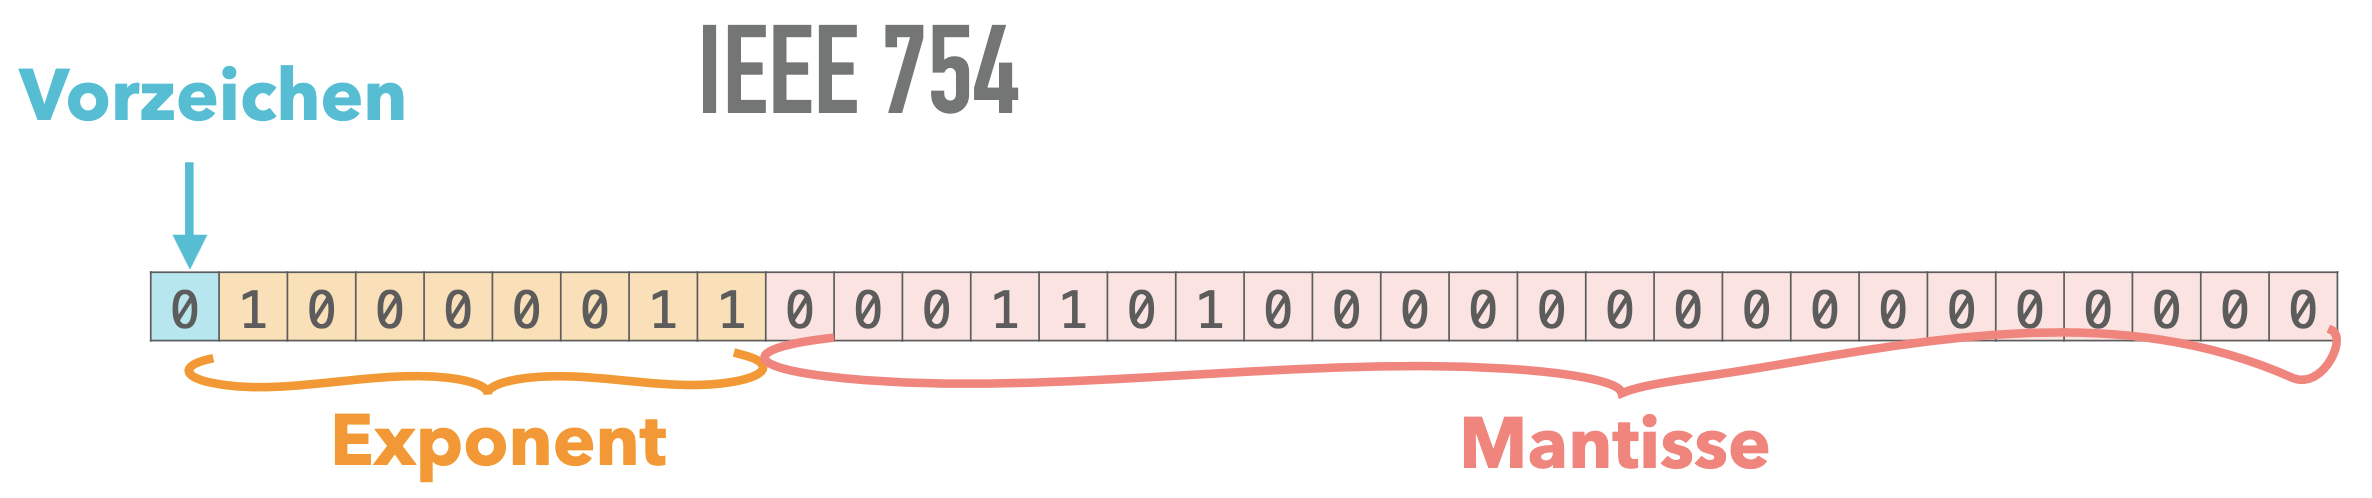
\includegraphics[scale=0.25]{Bilder/IEEE754.png} \\
		Wenn man eine Dezimalzahl in ein Floating Point umwandeln will muss man: 
		\begin{enumerate}
			\item{Die Zahl in Binär umwandeln: $17.625_{10} = 10001.101_2$}
			\item{Diese normalisieren: $1.0001101 * 2^4$}
			\item{Den Exponenten berechnen indem er zum Bias addiert wird: 4 + 127 = 131}
			\item{Den Bias + Exponent zu einer Binärzahl umgewandeln: $131_{10} \to 10000011_2$}
			\item{Diese drei Teile zusammenfügen.}
		\end{enumerate}
		\subsection{Textdarstellung}
		\subsubsection{ASCII}
		Zeichen werden ebenfalls kodiert. Der erste weit verbreitete Standard war der ASCII-Code. Ursprünglich 1963 für die USA entwickelt, fand es auch international Anwendung kann jedoch nur 127 Zeichen kodieren. Obwohl es mit einem Byte kodiert wird, werden nur 127 der 255 Zeichen verwendet. Das MSB hat verschiedene Anwendungsmöglichkeit: \\
		\begin{itemize}
			\item{Parität - Es kann für eine sehr rudimentäre Fehlererkennung bei der Übertragung genutzt werden. Wenn die Anzahl der gesetzten Bits somit gerade ist, ist das MSB 1, sonst 0. Dabei kann jedoch nur erkannt werden, dass es einen Fehler gibt und, falls es zwei Fehler gibt wird dieser nicht erkannt.}
			\item{In gewissen Erweiterungen werden die weiteren Zahlen auch um nicht englische Buchstaben erweitert.}
		\end{itemize}
		Man kann mit ASCII auch Bilder darstellen. Bei sogenannter ASCII-Art werden die 127 ASCII Zeichen verwendet um ein Bild rudimentär darzustellen.
		\subsubsection{Unicode}
		Unicode ist der heutzutage am weitesten verbreitete Standard zur Zeichenkodierung und beinhaltet zusätzlich Umlaute, kyrillische Schriftzeichen aber auch chinesische und Emojis. Es gibt unterschiedliche Wege Unicode zu kodieren wie z.B. UTF-8, LE-16 und andere. UTF-8 ist jedoch die beliebteste. UTF-8 hat den Vorteil, dass die Bytekodierung die selbe ist als ASCII bei Zeichen unter 128. Zusätzlich ist UTF-8 variabel und kann zwischen einem und 4 Bits verwenden. Abhängig davon wie viele Zeichen kodiert werden müssen mehr Zeichen angegeben werden, was sehr platzsparend ist. \\
		UTF-8 gibt am Anfang stets an wie viele Byte das System pro Zeichen erwarten muss. So hat das Erste Byte eine Bitfolge 11 und jedes Nachfolgebyte eine Zahlenfolge von 10. \\
		So steht bei ASCII Zeichen am Anfang eine 0 und danach die 7 Bits des ASCII Zeichens: \textbf{0}000007F. Wenn mehr als ASCII verwendet wird, stehen eine variable Menge an Bytes zu Verfügung, wobei im ersten byte jeweils die Anzahl der Einsen anzeigt wie viele Byte danach zu erwarten sind. \\
		Zum Beispiel wenn drei Bytes verwendet werden: 111xxxxx 10xxxxxx 10xxxxxx.
		\subsection{Bild- und Tondarstellung}
		Bilder werden ebenfalls aus Bytes dargestellt. Bitmap Bilder wie JPEG und PNG werden aus Pixeln zusammengestellt, dabei wird jeder Pixel durch einen Binärwert dargestellt. Videos werden auf ähnliche Weise dargestellt, wobei in den rudimentärsten Videos viele Bilder schnell hintereinander angezeigt weren. \\
		Ton ist eine Schallwelle, welches ebenfalls abgetastet und digitalisiert werden kann. Dabei ist die Abtastrate, die Rate wie oft die Schallwelle analysiert wird, für die Qualität des Tons relevant. Ebenfalls ist die Bittiefe wichtig, wodurch die Hertzrate der Welle genauer wiedergegeben werden kann.
		\section{Logik}
		\subsection{Logikgatter}
		Die Boolsche Algebra, benannt nach George Boole, beschreibt eine spezielle algebraische Struktur, in welcher es nur zwei Möglichkeiten gibt: Wahr und Falsch. Das praktische ist, dass ein solcher Wahrheitsgehalt mit nur einem Bit dargestellt werden können. In der Boolschen Logik gibt es viele Operatoren, unter anderem: NOT ($\neg$), AND($\land$), OR($\lor$). \\
		\begin{itemize}
			\item{Bei NOT wird der momentane Wahrheitswert invertiert, also wird Wahr zu Falsch und Falsch zu Wahr.}
			\item{Bei AND müssen beide Werte Wahr sein, sonst ist es Falsch.}
			\item{Bei OR ist das Ergebnis hingegen nur Falsch wenn beide Werte Falsch sind.}
		\end{itemize}
		Da ein Bit einen logischen Wert darstellen kann, kann man Bits auch als eine Folge logischer Werte interpretieren. \\ \\
		\begin{tabular}{l|c|c|c|c|c|c|c|c}
			NOT&1&0&1&1&0&1&0&$1_2$ \\ \hline
			Ergebnis&0&1&0&0&1&0&1&$0_2$
		\end{tabular} \\ \\
		So kann man eine Bitfolge anhand seiner Wünsche manipulieren:
		\begin{itemize}
			\item{Bei einem NOT wird die Bitfolge negiert.}
			\item{Bei einem AND kann man einen Teil einer Bitfolge anhand einer anderen auf 0 setzen oder 'maskieren' (mask on)}
			\item{Bei einem OR kann man einen Teil einer Bitfolge anhand einer anderen auf 1 setzen oder 'demaskieren' (mask off)}
		\end{itemize}
		\subsection{Kombinatorische Schaltungen}
		Ein jedes elektrisches System kann auf diese drei Logikgatter zurückgeführt werden. Jede Operation auf einem PC, ob es Musik, Audio oder Spiele sind, werden in ihren elementarsten Ebenen anhand von Logikgattern verarbeitet. \\
		Wenn man viele Logikgatter miteinander verknüft kann man, so alle Berechnungen ausführen. Man kann auch aus einfacheren Schaltungen komplexere bauen, wie zum Beispiel den XOR Schalter, welcher nur Wahr ist, wenn die beiden Inputs unterschiedlich sind:
		\begin{tabular}{| c | c | c |}
			\toprule
			A & B & Y \\ \midrule
			0 & 0 & 0 \\ \hline
			0 & 1 & 1 \\ \hline
			1 & 0 & 1 \\ \hline
			1 & 1 & 0 \\
			\bottomrule
		\end{tabular} \\ \\
		Ein anderes Bauteil ist der Halbaddierer (Half Adder), welcher zwei Binärzahlen zusammenfügen kann. Dieser wird ermöglicht indem wiederum ein XOR und ein AND Gatter miteinander verknüpft werden. \\
		Der Output eines Halbaddierers ist jeweils ein Bit sowie ein carry. Der Halbaddierer kann zwar diese Berechnung ausführen, jedoch nichts damit anfangen. Aus diesem Grund gibt es den Volladdierer, welcher aus zwei Halbaddierern mit einem zusätzlichen OR Gatter besteht und eine 1-Bit Zahl mit carry addieren kann. \\
		Wenn man vier dieser Volladdierer nun in Folge schaltet und dabei jeweils zwei Bits und einen carry in (falls vorhanden) aus der vorherigen Rechnung berücksichtigt, kann man so eine 4 Bit Zahl addieren kann. 
		\subsubsection{Sequenzielle Schaltungen}
		Diese Schaltungen nennt man Kombinatorische Schaltungen, welche nur einen Input haben und nicht in der Lage sind Information zu speichern und auch keine Zyklen besitzt. Diese Schaltungen dienen lediglich zur Verarbeitung von Information. \\
		Dazu gibt es die Sequenziellen Schaltungen, bei welchen der Ausgang zusätzlich von einem Input als auch einem früheren Output abhängt. Dadurch kann man Information aufbewahren und später wiedervwerwenden.
		\newpage
		\subsection{Merkblatt:}
		\textbf{Zahlensystem konvertieren:}
		\begin{itemize}
			\item{DEZ $\to$ HEX/BIN}
			\begin{itemize}
				\item{Dezimalzahl stets durch Basis (2 oder 16) teilen, Rest aufschreiben und Ergebnis erneut dividieren. Wenn das Ergebnis 0 ist, ist man fertig. Die Hex/Binärzahl ist der Rest von unten nach oben (Bei Hex Zahlen über 10 in A - F umwandeln.)}
			\end{itemize}
			\item{BIN $\to$ HEX}
			\begin{itemize}
				\item{Von links nach rechts jeweils 4 Binärzahlen gruppieren. Ist die Anzahl der Zahlen nicht durch 4 teilbar, können Nullen hinzugefügt werden. Da 4 Bits genau eine Hexadezimalzahl darstellen kann, sind 4 jeweils eine Zahl.}
			\end{itemize}
			\item{HEX $\to$ DEZ/BIN}
			\begin{itemize}
				\item{Stellenwertsystem: Jeder Ziffer in der Ursprungszahl einen Exponenten zuweisen. Die erste Zahl erhält eine 0 und jede darauffolgende 1 höher. Dann werden diese anhand der Formel ($Ziffer * [Basis]^{Exponent}$) addiert.}
			\end{itemize}
		\end{itemize}
		\textbf{Binär rechnen:}
		\begin{itemize}
			\item{Addition:}
			\begin{itemize}
				\item{Jede Ziffer der beiden Zahlen miteinander addieren: Wenn beide 0 sind wird es 0, wenn eines 1 ist, ist es 1 und wenn beide 1 sind, ist es 0 mit einem carry zur nächsten Ziffer. Diese Ziffer wird dann wieder zu dem nächsten Paar addiert.}
			\end{itemize}
			\item{Subtraktion:}
			\begin{itemize}
				\item{2s-Complement: Bei $a-b \to a+(-b)$ wird b zuerst invertiert und dann mit a addiert. Zur Negation wird eine Zahl gebitflipped (Alle 1 zu 0 und alle 0 zu 1) und an der LSB eine 1 addiert. Diese beiden Zahlen werden dann addiert.}
			\end{itemize}
			\item{Multiplikation}
			\begin{itemize}
				\item{Jede Ziffer wird mit jeder anderen Ziffer verundet. Beide 1 heißt 1, beide 0 heißt 0 und eine Ziffer 1 heißt auch 1. Nach jeder Ziffer wird der LSB danach um 1 nach Links gesetzt. Diese Produkte werden danach miteinander addiert.}
			\end{itemize}
		\end{itemize}
		\newpage
		\section{Aussagenlogik}
		\subsection{Syntax}
		In der klassischen Aussagenlogik gibt es zusätzlich zu Konstanten wie falsch oder wahr, auch Symbole (Auch Atome genannt), welche eine gewisse Aussage tätigen können. Ein Symbol kann auch ein Literal sein, wodurch es entweder das Symbol oder dessen Negation ist. Diese Symbole können auch verbunden werden:
		\begin{itemize}
			\item{Negation $\to$ Das Gegenteil des Symbols}
			\item{Konjunktion $\to$ Nur Falsch, wenn beide Symbole falsch sind.}
			\item{Disjunktion $\to$ Nur Wahr, wenn beide Symbole wahr sind.}
			\item{Implikation $\to$ Nur Falsch wenn aus etwas wahrem etwas falsches gezogen wird. A Wahr, B Falsch}
			\item{Bijunktion $\to$ Nur wahr wenn beide Symbole gleich sind. Wahr/Wahr und Falsch/Falsch.}
		\end{itemize}
		Diese Operatoren haben, gleich wie in der Mathematik, eine Reihenfolge. Hier gilt die allgemeine Regel, dass unäre (Operatoren mit nur einem Argument) immer vor binären Operatoren ausgewertet werden:
		\begin{enumerate}
			\item{Negation $\neg$}
			\item{Konjunktion $\lor$}
			\item{Disjunktion $\land$}
			\item{Implikation $\implies $}
			\item{Bijunktion $\iff$}
		\end{enumerate}
		\subsection{Semantik}
		In der Aussagenlogik gibt es verschiedene Semantiken:
		\begin{itemize}
			\item{Erfüllbar}
			\begin{itemize}
				\item{Wenn mindestens eine Interpretation existiert, in welcher die Aussage wahr ist.}
			\end{itemize}
			\item{Unerfüllbar}
			\begin{itemize}
				\item{Wenn keine der Interpretationen wahr ist.}
			\end{itemize}
			\item{Gültig}
			\begin{itemize}
				\item{Tautologie. Eine Aussage die immer wahr ist.}
			\end{itemize}
			\item{Äquivalent}
			\begin{itemize}
				\item{Wenn zwei Aussagen stets die selbe Interpretation haben. (A und $\neg$($\neg$ A))}
			\end{itemize}
		\end{itemize}
		Es gibt auch spezielle Strukturen, welche gewisse aufweisen:
		\begin{itemize}
			\item{Klausel}
			\begin{itemize}
				\item{Nur Oder Verknüpfungen}
			\end{itemize}
			\item{Cube}
			\begin{itemize}
				\item{Nur Und Verknüpfung}
			\end{itemize}
			\item{Hornklausel}
			\begin{itemize}
				\item{Eine Aussage, in welcher nur ein Symbol keine Negation hat.}
			\end{itemize}
			\item{Konjunktive Normalform (KNF)}
			\begin{itemize}
				\item{Konjunktion von Disjunktionen $\to$ Außen nur Und und innen nur Oder}
			\end{itemize}
			\item{Disjunktive Normalform (DNF)}
			\begin{itemize}
				\item{Disjunktion von Konjunktionen $\to$ Außen nur Oder und innen nur Und}
			\end{itemize}
		\end{itemize}
		\subsection{Bool'sche Rechengesetze zur Vereinfachung}
		Die Bool'schen Rechenregeln legen die Grundsätze der Bool'schen Logik dar. Die meisten dieser Regeln sind für moderne Verhältnisse relativ offensichtlich.
		\begin{itemize}
			\item{Dualitätsgesetz}
			\begin{itemize}
				\item{Alle Aussagen die nicht wahr sind, sind falsch und alle Aussagen die falsch sind, sind nicht wahr.}
				\item{$\neg\top =\bot$}
				\item{$\neg\bot =\top$}
			\end{itemize}
			\item{Idempotenz}
			\begin{itemize}
				\item{Ein Symbol das mit sich selbst verundet oder verodert wird, ergibt das Symbol selbst.}
				\item{$a\land a=a$}
				\item{$a\lor a=a$}
			\end{itemize}
			\item{Doppelte Negation}
			\begin{itemize}
				\item{Zwei negative vorzeichen ergeben ein positives Vorzeichen.}
				\item{$\neg(\neg a) = a$}
			\end{itemize}
			\item{Komplementärgesetz}
			\begin{itemize}
				\item{Ein Symbol das mit sich selbst negativ ver\textbf{und}et wird, ist immer \textbf{Falsch}.}
				\item{$a\land\neg a = \bot$}
				\item{Ein Symbol das mit sich selbst negativ ver\textbf{oder}t wird, ist immer \textbf{Wahr}.}
				\item{$a\lor\neg a = \top$}
			\end{itemize}
			\item{Kommutativgesetz}
			\begin{itemize}
				\item{Die Reihenfolge der Symbole, welche mit Und/Oder verbunden werden, ist irrelevant}
				\item{$a\land b = b\land a$}
				\item{$a\lor b = b \lor a$}
			\end{itemize}
			\item{Neutralitätsgesetz}
			\begin{itemize}
				\item{Wenn ein Symbol mit \textbf{Falsch} ver\textbf{oder}t wird, ist das Ergebnis nur von dem Symbol abhängig.}
				\item{$a\lor\bot =a$}
				\item{Wenn ein Symbol mit \textbf{Wahr} ver\textbf{und}et wird, ist das Ergebnis nur von dem Symbol abhängig.}
				\item{$a\land\top = a$}
			\end{itemize}
			\item{Extremalgesetz}
			\begin{itemize}
				\item{Ein Symbol das mit \textbf{Wahr} ver\textbf{oder}t wird, ist immer Wahr.}
				\item{$a\lor\top =\top$}
				\item{Ein Symbol das mit \textbf{Falsch} ver\textbf{und}et wird, ist immer Falsch.}
				\item{$a\land\bot =\bot$}
			\end{itemize}
			\item{Absorptionsgesetz}
			\begin{itemize}
				\item{Ein Symbol a, verundet mit sich selbst oder einem anderen Symbol b ist nur von a abhängig.}
				\item{$a\land(a\lor b)=a$}
				\item{Ein Symbol a, verodert mit sich selbst und einem anderen Symbol b ist nur von a abhängig.}
				\item{$a\lor(a\land b)=a$}
			\end{itemize}
			\item{Assoziativgesetz}
			\begin{itemize}
				\item{Wenn drei Symbole mit den gleichen Operatoren verbunden werden, ist es egal welcher zuerst evaluiert wird.}
				\item{$a\lor(b\lor c)=(a\lor b)\lor c$}
				\item{$a\land(b\land c)=(a\land b)\land c$}
			\end{itemize}
			\item{Distributivgesetz}
			\begin{itemize}
				\item{Wenn ein Symbol mit zwei Symbolen in Klammer multipliziert werden, müssen diese ausmultipliziert werden. Dabei werden die Operatoren getauscht.}
				\item{$a \lor\ (b \land\ c) = (a\lor\ b) \land\ (a \lor\ b)$}
				\item{$a \land\ (b \lor\ c) = (a\land\ b) \lor\ (a \land\ b)$}
			\end{itemize}
			\item{De Morgan'sche Gesetze}
			\begin{itemize}
				\item{Wenn zwei Symbole in Klammer negiert werden, kann dies zu zwei negierten Symbolen mit einem negierten Operator simplifiziert werden}
				\item{$\neg (x \lor\ y) = \neg x \land\ \neg y$}
				\item{$\neg (x \land\ y) = \neg x \lor\ \neg y$}
			\end{itemize}
		\end{itemize}
		Zwei Gesetze, welche nicht explizit zu den Bool'schen Gesetzen gehören, jedoch auch Anwendung finden:
		\begin{itemize}
			\item{Elimination von $\iff$ }
			\begin{itemize}
				\item{Man kann ein $\iff$ in zwei verundete Implikationen spalten}
				\item{$a \iff\ b = (a \implies\ b) \land\ (b \implies a)$}
			\end{itemize}
			\item{Elimination von $\implies$}
			\begin{itemize}
				\item{Eine Implikation kann zu einem negierten a mit verodertem b simplifiziert werden.}
				\item{$a \implies b = \neg a \lor\ b$}
			\end{itemize}
		\end{itemize}
		Übung: \\
		\begin{tabular}{lc}
		$a \implies\ (b \land\ a)$ & Implikationselimination \\
		$\neg a \lor\ (b \land\ a)$ & Distributivgesetz \\
		$(\neg a \lor\ b) \land\ (\neg a \lor\ a)$ & Komplementärgesetz \\
		$(\neg a \lor\ b) \land\ \top$ & Neutralitätsgesetz \\
		$(\neg a \lor\ b)$ & \\
		\end{tabular}
		\subsubsection{Erfüllbarkeitsproblem}
		Ein NP-Vollständiges Problem der Aussagenlogik, ist das Erfüllbarkeitsproblem, welches fragt, ob eine aussagenlogische Formel so belegt werden kann, dass sie wahr ist. Während die Lösung einer Formel mit drei Operanden noch relativ einfach ist, hat dasselbe Problem mit tausend Operanden eine viel höhere Schwierigkeit. \hyperref[sec:Komplexität]{\underline{(Siehe NP-Complete)}} \\
		Diese Probleme sind nur geschlossen lösbar, wenn diese zur Horn-Formel umformbar sind.
		\subsubsection{Merkblatt}
		\begin{tabular}{| c | c |}
			\toprule
			Name & Regel \\ \midrule
			Komplementärgesetz & $a\lor\neg a=\top$ \\
			&$a\land\neg a=\bot$ \\ \hline
			Kommutativgesetz & $a\lor b=b\lor a$\\
			&$a\land b=b\land a$ \\ \hline
			Dualitätsgesetz & $\neg\top=\bot$\\
			&$\neg\bot=\top$ \\ \hline
			Idempotenz & $a\lor a=a$\\
			&$a\land a=a$ \\ \hline
			Doppelte Negation & $\neg(\neg a)=a$ \\ \hline
			Neutralitätsgesetz & $a\lor\bot=a$\\
			&$a\land\top=a$ \\ \hline
			Extremalgesetz & $a\lor\top=\top$\\
			&$a\land\bot=\bot$ \\ \hline
			Absorptionsgesetz & $a\land(a\lor b)=a$ \\
			&$a\lor(a\land b)=a$ \\ \hline
			Assoziativgesetz & $a\textcolor{red}{\lor} (b\textcolor{red}{\lor} c)=(a\textcolor{red}{\lor} b)\textcolor{red}{\lor} c$ \\
			&$a\textcolor{blue}{\land} (b\textcolor{blue}{\land} c)=(a\textcolor{blue}{\land} b)\textcolor{blue}{\land} c$ \\ \hline
			Distributivgesetz & $a\textcolor{red}{\lor} (b\textcolor{blue}{\land} c)=(a\textcolor{red}{\lor} b)\textcolor{blue}{\land} (a\textcolor{red}{\lor} c)$ \\
			&$a\textcolor{blue}{\land} (b\textcolor{red}{\lor} c)=(a\textcolor{blue}{\land} b)\textcolor{red}{\lor} (a\textcolor{blue}{\land} c)$ \\ \hline
			De Morgan'sches Gesetz & $\neg(a\land b)=\neg a\lor\neg b$ \\
			&$\neg(a\lor b)=\neg a\land\neg b$ \\ \hline
			$\iff$ Elimination & $a\iff b=(a\implies b)\land(b\implies a)$ \\ \hline
			$\implies$ Elimination & $a\implies b=(\neg a\lor b)$ \\
			\bottomrule
		\end{tabular} \\
		Normalformen:
		\begin{itemize}
			\item{\textcolor{blue}{Konjunktive} Normalform (KNF)}
			\begin{itemize}
				\item{\textcolor{blue}{Konjunktion} von \textcolor{red}{Disjunktionen} (Außen \textcolor{blue}{und}, innen \textcolor{red}{oder})}
				\item{$a\textcolor{blue}{\land} (b\textcolor{red}{\lor} c)$}
			\end{itemize}
			\item{\textcolor{red}{Disjunktive} Normalform (DNF)}
			\begin{itemize}
				\item{\textcolor{red}{Disjunktion} von \textcolor{blue}{Konjunktionen} (Außen \textcolor{red}{oder}, innen \textcolor{blue}{und})}
				\item{$a\textcolor{red}{\lor} (b\textcolor{blue}{\land} c)$}
			\end{itemize}
		\end{itemize}
		\newpage
		\section{Von Neumann Architektur}
		Bevor die Von Neumann Architektur verbreitet war, gab es keinen weit verbreiteten Standard zur Architektur von Computern (Welche noch ganze Stockwerke ausfüllten). In der Von Neumann Architektur werden das Programm und die Eingabedaten im gleichen Speicher gespeichert. So musste man nicht mehr mit fixer Verkabelung arbeiten sondern das Programm individuell anpassen. \\
		John von Neumann beschrieb 1945 eine Architektur für eine allgemein einsetzbare Rechenanlage. \\
		Er beschrieb Komponenten eines Systems welches zusammenarbeiten sollten:
		\begin{itemize}
			\item{CPU (Steuerwerk und Rechenwerk)}
			\item{Bus-System}
			\item{Ein/Ausgabewerk}
			\item{Speicherwerk}
		\end{itemize}
		\subsection{Speicherwerk}
		Das Speicherwerk ist grundlegend nur eine Anzahl an Zellen, welche einen Inhalt speichern können. Jede dieser Zellen hat die gleiche Größe(In den meisten modernen Systemen 64-Bit). Diese Zellen sind entweder befüllt oder nicht befüllt. Der RAM eines jeden Computers nimmt den Platz des Speicherwerks ein. Das Gegenstück zum RAM (Random Access Memory) ist das Sequential Access Memory, wie zum Beispiel eine Kassette, in welchem man durch den Speicher gehen muss, um an eine bestimmte Information zu kommen. Der RAM kann jede Zelle in dem Speicher direkt ansprechen ohne abhängig von den anderen Zellen zu sein. RAM ist auch flüchtig und verliert seinen Speicher, wenn keine Energie vorhanden ist. Der Gegensatz zu diesem flüchtigen Speicher ist der persistente Speicher wie eine Festplatte oder eine SSD. \\
		Da im Speicherwerk sowohl das Programm als auch die Daten liegen, muss man aufpassen, dass man nicht unabsichtlich das Programm überschreibt. Normalerweise stellt jedoch das Betriebssystem sicher, dass Programmspeicher und Datenspeicher nicht in Konflikt kommen. Ein Programm ist im Speicher als Folge von Befehlen gespeichert, welches sequentiell ausgeführt wird.
		\subsection{Rechenwerk/CPU}
		Das Rechenwerk ist der zentrale Teil des Systems, in welcher alle Befehle abgearbeitet werden. Es verarbeitet die Befehle sequentiell anhand ihres Codes. Eine CPU besteht aus mehreren Komponenten:
		\begin{itemize}
			\item{Register}
			\begin{itemize}
				\item{Ein in die CPU integrierter kleiner Speicher, welcher als sehr schnell verwendbarer Zwischenspeicher für die CPU agieren kann.}
			\end{itemize}
			\item{Control Unit}
			\begin{itemize}
				\item{Regelt den Ablauf der CPU und stellt sicher, dass alle Aufgaben abgearbeitet werden. Solche Koordinationsaufgaben sind z.B. Befehle aus dem Speicher holen.}
				\item{Das Control Unit zählt mit, welche Zeile des Programms ausgeführt wurde um bei dem nächsten Befehl nicht den selben auszuführen. Ein weiterer Zwischenspeicher ist das Instruction Register um die momentane Operation festzuhalten.}
			\end{itemize}
			\item{ALU}
			\begin{itemize}
				\item{Vollführt die arithmetischen Operationen wie addieren, subtrahieren, inkrementieren (Um 1 erhöhen), dekrementieren (Um 1 verringern) und kann auch logische Operationen ausführen wie Vergleichsoperationen.}
				\item{Eine ALU besteht üblicherweise aus zwei Inputs, einem Output sowie einem OP-Code. Mittels des Inputs werden die zwei Zahlen eingelesen und anhand des OP-Codes verarbeitet und an den Output weitergegeben.}
				\item{Eine ALU hat auch ein Statusregister, welches gewisse Stati speichern kann. So kann festgestellt werden, dass bei einer Addition ein Overflow entsteht und das weitergegeben werden muss. Andere oft vorhandene register sind ein Output der Null ergibt, sowie ein Output der negativ ist. Diese Flags werden dann an das Control Unit weitergegeben.}
			\end{itemize}
		\end{itemize}
		Die CPU verwendet so das Steuerwerk und Rechenwerk um die Befehle abzuarbeiten und auszuwerten. Der Ablauf kann wie folgt aussehen: 
		\begin{enumerate}
			\item{Hole den Inhalt aus einer Speicherzelle und speichere ihn in einem Register.}
			\item{Hole den zweiten Inhalt aus einer Speicherzelle und speichere ihn auch in einem Register.}
			\item{Aktiviere die Additionseinheit mit dem Inhalt der beiden Registern als Eingabe und speichere das Ergebnis in einem weiteren Register.}
			\item{Speichere das Resultat in einer Speicherzelle.}
		\end{enumerate}
		\subsection{Bus-System}
		Damit Information vom RAM in die CPU übertragen werden kann, muss dieses übertragen werden. Das passiert mithilfe des Bus-Systems. Das Bus-System ist ein exklusives Betriebsmittel und es kann zu einem Datenstau kommen, wenn zu viel Informatiom übertragen wird. Einige Busarten sind:
		\begin{itemize}
			\item{Datenbus - Verbindet die CPU mit dem Arbeitsspeicher}
			\item{Adressbus - Überträgt eine Speicheradresse}
			\item{Steuerbus - Übermittelt Steuerinformationen (Ob Lesen oder Schreiben)}
		\end{itemize}
		Das Bus-system hat eine Wortbreite, was die maximale Anzahl an Bits definiert, welche gleichzeitig übertragen werden können.
		\subsection{Ein-/Ausgabewerk}
		Das Ein-/Ausgabewerk ist die gesamte Peripherie, mit welcher Information von und zu dem PC ausgegeben und eingegeben werden kann. Das kann eine Tastatur, eine Maus aber auch eine Festplatte sein.\\
		Dabei braucht jedes Gerät Kontrollsoftware (Treiber) um mit dem PC interagieren zu können. Diese bilden die Schnittstelle zwischen dem Gerät und dem PC. Ein Treiber ist oft spezifisch für einen Hersteller, also gibt es keine universellen Treiber.
		\subsection{Harvard- und Von Neumann-Architektur}
		In der Harvard Architektur sind Daten und Programm nicht im selben Speicherwerk gespeichert. So existiert ein Programm- und ein Datenspeicher. Der Vorteil dieser Architektur ist, dass gleichzeitig Daten und Programme geladen oder geschrieben werden können. So sind auch die Datenwortbreite und die Programmwortbreite unabhängig voneinander. \\
		Ein weiterer Aspekt ist die erhöhte Sicherheit, da nicht fälschlicherweise Daten als Programm interpretiert werden können. \\
		Jedoch muss es zwei separate Speicher geben, wodurch ungenutzter Speicher in einem oder dem anderen nicht anderweitig verwendet werden kann.
	\section{Sprachen}
	\subsection{Was ist Sprache?}
	Sprachen sind ein Mittel der Kommunikation, welche gewisse Regeln vorraussetzt. Zum Beispiel benötigt man ein Fragezeichen um eine Frage darzustellen. Dabei gibt es auch Regeln, wie zum Beispiel, dass ein Fragzeichen nur am Ende eines Satzes vorkommen kann. \\
	Auch Programmiersprachen folgen Sprachregeln, sind jedoch bedeutend präziser. Während menschliche Sprachen oft mehrdeutig sind und sich auch verändern, bleiben formale Sprachen meist gleich und bieten Präzision. \\
	\subsection{Syntax und Semantik}
	Syntax beschreibt welche Ausdrücke zu einer Sprache gehören und die Regeln nach welchen Sätze gebildet werden können. Semantik hingegen legt fest was Wörter bedeuten und ob die Zusammensetzung der Wörter einen Sinn ergibt. Zum Beispiel ist der Satz "Der Hase lenkte den Mond gestern in der Bibliothek." syntaktisch gesehen einwandfrei, semantisch gesehen jedoch fragwürdig. \\
	Syntax und Semantik sind auch in Programmiersprachen relevant. \\
	\begin{verbatim}
	public int my_foo ( {
		int i = "abced";
	}
	\end{verbatim}
	In diesem Codebeispiel findet man sowohl semantische als auch syntaktische Fehler. Die öffnende Klammer in Zeile 1 ohne schließendes Gegenstück, ist ein syntaktischer Fehler. Der Versuch einer Integervariable einen String zuzweisen ist jedoch ein Semantischer. Syntaktik überprüft somit ob der Code die korrekte Struktur während Semantik überprüft, ob Deklarationen und Anweisungen die korrekte Struktur haben. \\
	\subsection{Definition einer Sprache}
	Formale Sprachen werden durch spezifische Zeichen definiert:
	\begin{itemize}
		\item{Alphabet ($\Sigma$)}
		\begin{itemize}
			\item{Das Alphabet stellt eine nicht leere (Muss mindestens ein Zeichen enthalten), endliche (Hat eine klar definierte Menge) Menge an Zeichen und Symbolen dar.}
			\item{Das Deutsche Alphabet kann man zum Beispiel als $\Sigma$=\{a,b,...,z,A,...,Z,Ü,...\} dargestellt werden.}
		\end{itemize}
		\item{Zeichenkette/Wörter}
		\begin{itemize}
			\item{Endliche Kette an Zeichen aus dem Alphabet}
		\end{itemize}
		\item{Leerwort $\epsilon$}
		\begin{itemize}
			\item{Ein Wort, welches kein Zeichen enthält.}
		\end{itemize}
		\item{Sprache \textbf{L}}
		\begin{itemize}
			\item{Eine bestimmte Teilmenge aller möglichen Wörter, welche mit dem Alphabet dargestellt werden kann.}
			\item{Jede Zeichenkette, welche nur Symbole aus der spezifischen Sprache enthält, ist Teil der Sprache.}
		\end{itemize}
	\end{itemize}
	\subsection{Noam Chomsky's Sprachhierachie}
	Noam Chomsky beschrieb 1956 die 4 Stufen der formalen Sprachen:
	\begin{itemize}
		\item{Reguläre Sprache}
		\item{Kontextfreie Sprachen}
		\item{Kontextsenitive Sprachen}
		\item{Rekursiv aufzählbare Sprachen}
	\end{itemize}
	Jede dieser Sprachen beinhaltet die vorherigen, also beinhaltet eine rekursiv aufzählbare Sprache auch reguläre Sprachen. \\
	Auf diese wird später noch eingegangen. \hyperref[sec:Sprachhierarchie]{\underline{(Siehe Sprachhierarchie)}}
	\subsection{Reguläre Ausdrücke}
	Reguläre Ausdrücke werden folgerndermaßen definiert: \\
	Wenn $a \in \Sigma$ dann sind $\epsilon$ und a reguläre Ausdrücke.\\
	Wenn a und b reguläre Ausdrücke sind, dann sind auch folgende Ausdrücke reguläre Ausdrücke:
	\begin{itemize}
		\item{a | b}
		\begin{itemize}
			\item{Alternative - a oder b}
		\end{itemize}
		\item{ab}
		\begin{itemize}
			\item{Verkettung - Zuerst a, dann b}
		\end{itemize}
		\item{a*}
		\begin{itemize}
			\item{Kleene Stern - a kommt 0 mal oder öfter (Bis unendlich) vor (0 mal oder öfter)}
		\end{itemize}
		\item{a+}
		\begin{itemize}
			\item{Positive Hülle - a kommt 1 mal oder öfter (Bis unendlich) vor (1 mal oder öfter)}
		\end{itemize}
		\item{a?}
		\begin{itemize}
			\item{Optionaler Quantor - a kommt 0 oder 1 mal vor (Optional)}
		\end{itemize}
	\end{itemize}
	\paragraphlb{Beispiel:}
	In einem Alphabet $\Sigma = \{a,b\}$ kann man Ausdrücke folgend schreiben:
	\begin{itemize}
		\item{a | b = \{a,b\}}
		\item{a* = \{$\epsilon$, a, aa, aaa, ...\}}
		\item{(a | b)* = \{$\epsilon$, a, b, ab, aa, ...\}}
		\item{a+ = \{a, aa, aaa, aaaa, ...\}}
		\item{a? = \{$\epsilon$, a\}}
		\item{a(b | a) = \{ab, aa\}}
	\end{itemize}
	\subsubsection{Reguläre Definitionen}
	Man kann einem regulären Ausdruck auch einen Namen geben um anschließend diesen Namen zu verwenden. Die Sequenz dieser Form kann so wiedergegeben werden: \\
	$d_1 \to r_1$ \\
	$d_n \to r_n$ \\
	So beschreibt die Definition \textbf{letter} alle englischen Buchstaben $\to$ $letter \to |A|...|Z|a|...|z|$\\
	Mit regulären Definitionen kann man reguläre Ausdrücke bedeutend leserlicher machen, da Ausdrücke oft sehr lang sein können. Wenn man so Ausdrücken zuerst Namen gibt und diese danach als Referenz verwendet, sind diese bedeutend einfacher zu lesen und entziffern. \\

	\section{Automaten}
	Jede reguläre Sprache kann durch einen regulären Ausdruck beschrieben werden. Eine reguläre Sprache kann jedoch auch durch einen endlichen Automaten beschrieben werden.
	\subsection{Deterministische Endliche Automaten (DFA)}
	Ein endlicher deterministischer Automat (DFA) ist eine Respräsentation eines regulären Ausdrucks, welcher von einem PC abgearbeitet werden kann. Ein Automat wechselt immer anhand einer Aktion den Zustand. \\
	\begin{figure}[H]
	\centering
	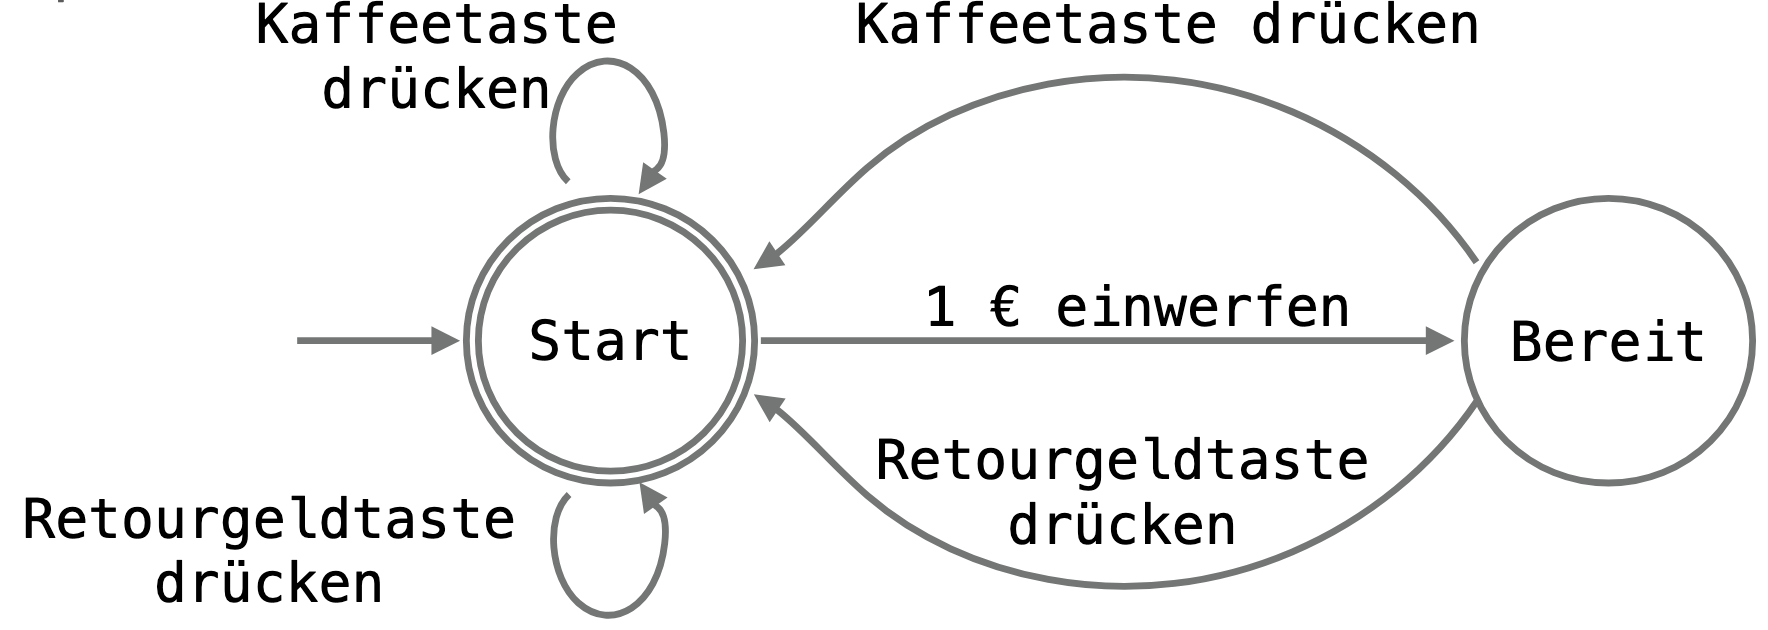
\includegraphics[scale=0.3]{Bilder/DFA.png}
	\caption{Repräsentation eines Kaffeeautomaten als endlicher Automat.}
	\end{figure}
	Ein Kaffeeautomat kann als endlicher Automat dargestellt werden, da er anhand eines inputs seinen Zustand verändert. \\
	\subsubsection{Definition}
	Ein endlicher Automat hat stets eine endliche Menge an Zuständen. Dabei gibt es weitere, spezielle Arten von Zuständen:
	\begin{itemize}
		\item{Startzustand: z0}
		\begin{itemize}
			\item{Der Zustand in welchem, der Automat beginnt. Wird markiert durch einen Pfeil (Kante) ohne Anfangszustand.}
		\end{itemize}
		\item{Endzustand: E}
		\begin{itemize}
			\item{In jedem Automaten gibt es eine Anzahl an Endzuständen, wobei Endzustände stets eine Teilmenge der Gesamtzustände sind. Endzustände werden durch doppelte Ränder gezeigt.}
		\end{itemize}
		\item{Alphabet der Eingabemenge: $\Sigma$}
		\begin{itemize}
			\item{Beinhaltet eine endliche, nicht leere Menge. Dieses Alphabet definiert die Arten von Übergängen die es geben kann.}
		\end{itemize}
	\end{itemize}
	Die Übergänge eines Automaten werden in einer Übergangstabelle festgehalten. Die Übergangstabelle definiert, welcher Zustand von dem jetzigen Zustand erreicht werden kann. Bei jeder Überschreitung einer Kante wird ein Eingabesymbol konsumiert. \\
	\begin{tabular}{| c | c | c |}
		\toprule
		& \textbf{0} & \textbf{1}  \\ \midrule
		z0 & e1 & e1 \\ \hline
		e1 & e1 & e1 \\
		\bottomrule
	\end{tabular} \\
	In dieser Tabelle wird die Übergangstabelle eines Automaten festgehalten. Dabei wird im Zustand z0 begonnen und bei Erhalten einer 0 oder 1, geht dieser in den Zustand e1 über. Wenn er danach noch eine 0 oder 1 erhält, bleibt er in Zustand e1. \\
	\subsubsection{Akzeptanz}
	Ein Automat akzeptiert ein Wort, wenn es bis zum Ende gelesen und vollständig konsumiert wurde. Ein Wort gilt als abgelehnt, wenn es nicht vollständig konsumiert worden ist, aber keine weiteren Übergänge möglich sind, oder nicht in einem Endzustand beendet wird, obwohl das Wort vollständig konsumiert wurde.
	\subsection{Nichtdeterministische Endliche Automaten (NFA)}
	Alle bisher angesehenen Automaten waren deterministische endliche Automaten. Dadurch ist der Pfad eines spezifischen Ausdrucks stets der selbe und vordeterminiert. Im Gegensatz dazu stehen Nicht-Deterministische Endliche Automaten, in welchen der nächste Schritt nicht im vorhinein bereits feststeht. Dadurch ist es möglich mehrere Wege für einen Zustandswechsel darzustellen. Es ist auch möglich eine leere Menge bei einem Zustandswechsel zu verwenden.
	\subsubsection{Grammatiken}
	Sprachen sind im allgemeinen unendlich, also enthalten sie unendlich viele Wörter und Kombinationen. Grammatiken können verwendet werden um diese unendlichen Sprachen endlich darzustellen. Das funktioniert auch im Deutschen, wo ein Subjekt, ein Objekt oder ein Artikel in einer Grammatik definiert sind. \\
	Dabei besteht ein Satz stets aus Terminalen und Nicht-Terminalen. Terminale sind statische Ausdrücke, welche den Endzustand des Satzes darstellen und auch als solche interpretiert werden sollten. Nicht-Terminale sind Komponenten eines Satzes, welche später durch andere Terminale oder Nicht-Terminale ersetzt werden. \\
	Eine Grammatik innerhalb einer formalen Sprache besteht aus:
	\begin{itemize}
		\item{Einer endlichen Menge an Nicht-Terminalen - $V_N$}
		\begin{itemize}
			\item{Dies entspricht in etwa der Menge an Zuständen der Grammatik und wird in der Regel großgeschrieben.}
		\end{itemize}
		\item{Einer endlichen Menge an Terminalen - $V_T$}
		\begin{itemize}
			\item{Entspricht dem Alphabet der Sprache und wird in der Regel kleingeschrieben.}
		\end{itemize}
		\item{Dem Startsymbol $S$, welches Teil der Nicht-Terminalen ist. (Initialzustand in einem Automaten)}
		\item{Einer endlichen Menge an Produktionsregeln - $P =\{\alpha \rightarrow \beta\}$ (Zustandsübergänge in einem Automaten.)}
	\end{itemize}
	Beispiel einer Grammatik zur Ableitung Binärer Zahlen: \\
	$V_N$ = \{S\}, $V_T$ = \{0, 1\}, S=S \\
	\begin{tabular}{l | l }
		\toprule
		\multicolumn{2}{c}{Regeln} \\ \midrule
		1. Regel & S $\rightarrow$ 0 \\ 
		2. Regel & S $\rightarrow$ 1 \\
		3. Regel & S $\rightarrow$ \underline{0}S \\
		4. Regel & S $\rightarrow$ \underline{1}S \\
		\bottomrule
	\end{tabular} \\
	Alternativ kann man diese Regeln auch als P = \{S $\rightarrow$ \underline{0} | \underline{1} | \underline{0}S | \underline{1}S\} angeben. \\
	
	Wenn man nun 10 ableiten will, muss man die Regeln anwenden, bis man entweder nur mehr Terminale zur Verfügung hat, oder keine Regel mehr ausführen kann (In welchem Fall es nicht Teil der Sprache ist.): \\
	10 ableiten :
	\begin{tabular}{ l  c  l  c  l }
		\toprule
		S &  $\Rightarrow$ & \underline{1}S & $\Rightarrow$ & \underline{10} \\ \midrule
		&4. Regel && 1. Regel \\
		\bottomrule
	\end{tabular} \\
	Also können Reguläre Sprachen auf drei verschiedene Weisen angegeben werden: Mit Regulären Ausdrücken, Automaten oder Regulären Grammatiken. Da diese in der gleichen Sprachhierarchie stehen, kann man eine stets in die andere übertragen. \\
	\subsubsection{Regulärer Ausdruck zu Regulärer Grammatik}
	Aus diesem Grund kann man den regulären Ausdruck \verb\a?(b|c)\  einfach in einer reguläre Grammatik übertragen: \\
	Wörter = \{b, c, ab, ac\} \\
	$V_N$ = \{S, Q\} \\
	$V_T$ = \{\underline{a}, \underline{b}, \underline{c}\} \\
	S = S \\ \\
	P = \begin{tabular}{ l | l }
		\toprule
		\multicolumn{2}{c}{Regeln} \\ \midrule
		1. Regel & S $\rightarrow$ \underline{a}Q \\
		2. Regel & S $\rightarrow$ $\epsilon Q$ \\
		3. Regel & Q $\rightarrow$ \underline{b} \\
		4. Regel & Q $\rightarrow$ \underline{c} \\
		\bottomrule
	\end{tabular}
	\subsubsection{Sprachhierarchie}
	\label{sec:Sprachhierarchie}
	Noam Chomsky definierte die Sprachen als Hierarchie anhand ihrer Mächtigkeit. Mit einer mächtigeren Sprache kann man so mehr Sprachen beschreiben. Jedoch ist dessen Verarbeitung auch komplexer. Die Einfachheit regulärer Ausdrücke hilft so effizient Text zu evaluieren.
	\begin{itemize}
		\item{Reguläre Sprachen}
		\begin{itemize}
			\item{Beschreibbar durch reguläre Ausdrücke, Automaten und Grammatiken}
			\item{Wortproblem effizient lösbar}
		\end{itemize}
		\item{Kontextfreie Sprache}
		\begin{itemize}
			\item{Beschreibbar durch kontextfreie Grammatiken}
			\item{Wortproblem effizient mit Kellerautomat (Stack) lösbar.}
			\item{Die meisten Programmiersprachen evaluieren input mittels kontextfreier Grammatik}
		\end{itemize}
		\item{Kontextsensitive Sprache}
		\begin{itemize}
			\item{Beschreibbar durch kontextsensitive Grammatiken}
			\item{Mit einer Turingmaschine lösbar, jedoch nicht effizient}
		\end{itemize}
		\item{Rekursiv aufzählbare Sprache}
		\begin{itemize}
			\item{Beschreibbar mittels einer Turingmaschine}
			\item{Wortproblem nicht in endlicher Zeit lösbar}
		\end{itemize}
	\end{itemize}
	\section{Turingmaschine}
	Ein Algorithmus beschreibt den konkreten Lösungsweg für ein Problem. So besteht ein Algorithmus aus endlich vielen Befehlen. \\
	David Hilbert definierte das Entscheidungsproblem, welches fragt, ob ein System zu einer gegebenen Aussage eine Entscheidung treffen kann, ob es wahr oder falsch ist. \\
	Das Wortproblem, ob zum Beispiel 'Haus' Teil der deutschen Sprache ist, ist auch ein Entscheidungsproblem. Wenn also in endlicher Zeit ihre Charakteristische Funktion: $X_L:w\rightarrow \{1,\ falls\ w\in L - sonst 0\}$ \\
	Dazu existiert noch das Komplement des Wortproblems, ist das Wort \textit{nicht} Teil der Sprache? \\
	Dabei muss man jedoch nicht nur zwischen Entscheidbar und Unentscheidbar unterscheiden, sondern auch zwischen der Semi-Entscheidbarkeit. \\
	Ein Problem ist Semi-Entscheidbar, wenn man zwar in endlicher Zeit herausfinden kann, dass ein Wort Teil der Sprache ist, das Programm jedoch unendlich lange läuft, wenn es nicht Teil der Sprache ist. Das Problem hierbei ist, dass eine unendlich lange Zeitspanne nicht definiert ist und man kann nie sicher sein, ob genug Zeit vollstrichen ist, um das Problem zu lösen oder es keine Lösung gibt. \\
	Eine Regel der Semi-Entscheidbarkeit ist, dass das Komplementär eines Semi-Entscheidbaren Algorithmuses nicht immer auch Semi-Entscheidbar ist. Jedoch ist ein Algorithmus Entscheidbar, wenn sowohl der Algorithmus als auch dessen Komplementär Semi-Entscheidbar sind. \\
	Ein Algorithmus ist jedoch Nicht Entscheidbar, wenn weder der positive, noch der negative Ausgang in positiver Zeit entschieden werden können.
	\subsection{Church-Turing These}
	Die CTT besagt, dass die Klasse der intuitiv berechenbaren Funktionen genau der Klasse der Turing-berechenbaren Funktionen entspricht. \\
	Die Turing Maschine ist ein Berechnungsmodell von Alan Turing und alles, was mit einer Turingmaschine berechnet werden kann, kann auch mit einer Programmiersprache berechnet werden. Wenn eine Programmiersprache die gleiche Funktion wie eine Turingmaschine hat, dann nennt man sie turing complete. Gleichzeitig gibt es jedoch keine Programmiersprache, welche mehr kann als eine Turingmaschine. \\
	Die Turingmaschine ist ein Berechnungsmodell, welche die Arbeitsweise eines Computers simuliert. Dadurch ist sie mathematisch einfach zu analysieren. Obwohl eine Turingmaschine eigentlich ein theoretisches Konzept ist, kann man es in eingeschränkter Weise nachbauen. Die Komponenten einer Turingmaschine sind:
	\begin{itemize}
		\item{Ein unendlich langes Band, welches beschrieben werden kann.}
		\item{Ein Schreib- und Lesekopf zum auslesen und beschreiben des Bandes.}
		\item{Ein Zwischenspeicher um den vorhin ausgelesenen Wert abspeichern zu können.}
		\item{Eine Übergangstabelle zur Definition von Zuständen.}
		\begin{itemize}
			\item{Die Tabelle hat ein bestimmtes Format: 1 RM 2}
			\begin{itemize}
				\item{Das Ausgabezeichen - 1}
				\item{Die Bewegung des Cursors - R (Rechts, Links oder gar nichts)}
				\item{Der neue Zustand - M2}
				\item{Zusätzlich wird für jeden ausgelesenen Wert ein eigener Zustand definiert.}
			\end{itemize}
		\end{itemize}
	\end{itemize}
	Eine Turingmascheine hat ebenfalls:
	\begin{itemize}
		\item{Eine endliche, nicht leere, Menge an Zuständen}
		\item{Einen Startzustand, sowie einen Endzustand}
		\item{Zusätzlich existieren der Akzeptanz- und der Ablehnungszustand, welcher entscheidet, ob positiv oder negativ entschieden wird.}
	\end{itemize}
	\subsection{Universelle Turingmaschine}
	Die universelle Turingmaschine (UTM) erweitert die Turingmaschine in der Weise, dass das Band zusätzlich ein Programm, also eine weitere Turingmaschine, enthält, welche von der Turingmaschine ausgeführt wird. Zusätzlich enthält das Band den Input, welcher von der UTM verarbeitet wird. \\
	Dies spiegelt die Idee der von Neumann Maschine, wieder, welche Programmcode und Daten auf dem gleichen Medium enthält.
	\subsubsection{Deterministische und Nicht Deterministische Turngmaschine}
	Ebenso wie bei Automaten gibt es auch Deterministische (DTM) und Nicht deterministische Turingmaschinen (NTM). Eine DTM hat stets den gleichen Pfad und besitzt für eine Eingabe nur eine Ausgabe. Eine NTM kann einen anderen Weg für die gleiche Lösung finden. Es ist nur wichtig, dass eine Lösung gefunden wird. \\
	\subsubsection{Halteproblem}
	\hyperdef{halteproblem1}{halteproblem2}
	Das Halteproblem ist die Frage, ob ein Programm den Quelltext eines anderen Programms erhalten kann um so zu entscheiden ob das Programm jemals beendet, oder nicht. Da eine Turingmaschine genauso mächtig ist wie eine Programmiersprache, kann man es auch auf diese andwenden und so überlegen, ob eine Turingmaschine entscheiden kann ob eine andere Turingmaschine als Input jemals anhält oder nicht. Alan Turing bewies, dass es für eine beliebige Turingmaschine nicht möglich ist diese Entscheidung zu treffen. \\
	Dabei spaltete er das Halteproblem in zwei Subhalteprobleme: \\
	Erstens soll H anhalten, wenn P mit Eingabe E anhält. H kann jedoch nicht wissen, wenn P nicht anhält, wodurch dieses Subproblem Semi-Entscheidbar ist. \\
	Weiters gibt es das Komplement dieses Problems, also,dass H anhalten soll, wenn P mit Eingabe E \textit{nicht} anhält. Diese Frage ist wiederum unentscheidbar, da H nie im vorhinein wissen kann, dass P unendlich lange läuft. \\
	Da eines der beiden Probleme unentscheidbar ist, ist das Halteproblem somit auch als ganzes Unentscheidbar.
	\section{Komplexität}
	\label{sec:Komplexität}
	Komplexität bezeichnet den Zeitaufwand, welcher ein spezifischer Algorithmus abhängig von der Größe \verb|n| des inputs zum Abschluss benötigt. Der Zeitaufwand eines Suchalgorithmuses ist abhängig von der Position des gesuchten Elements. Es kann in der ersten Position stehen, wodurch es nur eine Iteration benötigt, oder in der letzten, wobei der Algorithmus dadurch durch das gesamte Array iterieren muss. Es kann auch passieren, dass das Element überhaupt nicht vorhanden ist. Bei der Komplexität geht man stehts von dem schlechtestmöglichen Ergebnis, also würde ein Suchalgorithmus, welcher eine Position nach der anderen durchkämmt, eine lineare Komplexität abhängig von der Größe des Arrays. Dabei wird die Komplexität meist in der Landau Notation angegeben, welche asymptotisches Verhalten einer Funktion darstellt. Dadurch ist sie unabhängig von Maschine oder Dateneigenschaft. Man nennt diese Notation auch Big-O Notation (O(n) für eine lineare Komplexität). \\
	Bei der O Notation werden elementare Schritte gezählt. Diese inkludieren Zuweisungen, Arithmetische Operationen oder Vergleiche. Dabei benötigt jeder Schritt eine konstante Zeit. Größter Faktor der Notation ist jedoch die Anzahl der Elemente, welche durch \verb|n| angegeben werden. Dieses n ist abhängig von der Laufzeit, welche durch mehrere Klassen definiert ist:
	\begin{itemize}
	 	\item{Konstante Laufzeit}
	 	\begin{itemize}
	 		\item{Der Algorithmus ist unabhängig von der Anzahl der Elemente und hat stets die gleiche Laufzeit. - O(1)}
	 	\end{itemize}
	 	\item{Logarithmische Laufzeit}
	 	\begin{itemize}
	 		\item{Eine Verdoppelung des n, führt nur zu einem linearen Anstieg der Laufzeit. - O(log(n))}
	 	\end{itemize}
	 	\item{Lineare Laufzeit}
	 	\begin{itemize}
	 		\item{Bei Verdoppelung des n, verdoppelt sich auch die Laufzeit. - O(n)}
	 	\end{itemize}
	 	\item{Quadratische Laufzeit}
	 	\begin{itemize}
	 		\item{Bei einer Verdoppelung des n wächst die Laufzeit um das Vierfache. - O($n^2$)}
	 	\end{itemize}
	 	\item{Polynomielle Laufzeit}
	 	\begin{itemize}
	 		\item{Für jedes n, wächst die Laufzeit ungefähr um $2^m$. - O($n^m$)}
	 	\end{itemize}
	 	\item{Exponentielle Laufzeit}
	 	\begin{itemize}
	 		\item{Für jedes n verdoppelt sich die Laufzeit. - O($2^n$)}
	 	\end{itemize}
	 	\item{Faktorielle Laufzeit}
	 	\begin{itemize}
	 		\item{Für jedes n steigt die Laufzeit um das (n+1)fache. - O(n!)}
	 	\end{itemize}
	 \end{itemize} 
	 Diese Laufzeit wird normalerweise in O-Notation angegeben. Die grundlegende Formel beschreibt: $P(g(n))=\{f(n)|\exists c\in \N, \forall n \geq n_0: f(n)\leq c*g(n)\}$, was aussagt, dass eine Funktion \textit{g(n)} existiert, welche ab einem bestimmten Multiplikator \textit{c} immer größer (also langsamer) ist als eine andere Funktion \textit{f(n)}. \\
	 Indem man die Algorithmen vergleicht und so in Komplexitätsklassen teilt, kann man den Ressourcenbedarf eines Algorithmus' unabhängig vom System oder der Programmiersprache vergleichen. \\
	 Dabei kann man zwischen Zeit- und Speicherkomplexität unterscheiden. Größtenteils ist jedoch die Speicherkomplexität relevant. \\
	 \subsection{P vs NP}
	 Die Church-Turing-These besagt, dass jedes Programm, das berechenbar ist, in endlicher Zeit auch lösbar ist. Hier muss man jedoch zwischen Berechenbarkeit und Lösbarkeit unterscheiden. Jedes Problem ist \textit{lösbar}, jedoch ist die Frage nach welcher Zeit sie lösbar ist. Wenn ein Problem einen zu großen Aufwand zur Lösung bietet, nennt man diese Probleme berechenbar. \\
	 Zusätzlich unterscheidet man zwischen den \textbf{P} und den \textbf{NP} Problemen. \\
	 \textbf{P} Probleme haben einen effizienten Algorithmus mit dem das Problem gelöst werden kann. Alle Probleme, welche in zumindest polynomieller Zeit ($n^k$) gelöst werden können, gelten als \textbf{P}. Das inkludiert Algorithmen zum Sortieren oder der Bestimmung einer Primzahl. \\
	 Gegenseitig davon gibt es die \textbf{NP} Probleme, welche als nicht in polynomieller Zeit lösbar gelten. Es gibt zwar Algorithmen zur Berechnung dieser Probleme, diese sind jedoch extrem ineffizient. Theoretisch sind sie in einer Nicht-Deterministischen Turingmaschine in polynomieller Zeit berechenbar, falls man ein Orakel (Einen Weg, in jedem Fall die richtige Entscheidung zur Findung der Lösung zu finden.). Obwohl das Finden der Lösung schwer ist, ist die Verifizierung der Lösung jedoch relativ einfach. (Herausfinden ob die Lösung richtig ist.) In der Gruppe der \textbf{NP} Probleme gibt es noch die Untergruppe der \textbf{NP Kompletten (NP-C)} Probleme. Diese Probleme bieten die gleiche Komplexität als das Entscheidungsproblem und gelten als die schwersten lösbaren Probleme. Eine grundlegende Frage der Komplexität ist dabei, ob P und NP in der gleichen Klasse existieren. Diese Frage nennt man \verb|P=NP Problem| und versucht zu ergründen ob alle Probleme, welche in polynomieller Zeit verifizierbar sind, auch in gleicher Zeit gelöst werden können.
\end{document}